% !TeX spellcheck = en_US
% !TeX program = lualatex
\documentclass[14pt, aspectratio=169, sectionpage=simple, xclolor=table]{beamer}
\usetheme{emctria}
\usepackage{colortbl}
\usepackage{fancyvrb}
\usetikzlibrary{calc,fadings,shapes.arrows,shadows,backgrounds, positioning}
\usepackage{adjustbox}
\usepackage{xcolor}
\usepackage{adjustbox}
\usepackage{verbatim}
\usepackage{listings}

\setlength{\unitlength}{1cm}
\newcommand{\ba}{\mbox{{\boldmath $a$}}}
\newcommand{\bA}{\mbox{{\boldmath $A$}}}
\newcommand{\bb}{\mbox{{\boldmath $b$}}}
\newcommand{\bB}{\mbox{{\boldmath $B$}}}
\newcommand{\bc}{\mbox{{\boldmath $c$}}}
\newcommand{\bC}{\mbox{{\boldmath $C$}}}
\newcommand{\bd}{\mbox{{\boldmath $d$}}}
\newcommand{\bD}{\mbox{{\boldmath $D$}}}
\newcommand{\be}{\mbox{{\boldmath $e$}}}
\newcommand{\bE}{\mbox{{\boldmath $E$}}}
\newcommand{\bbf}{\mbox{{\boldmath $f$}}}
\newcommand{\bF}{\mbox{{\boldmath $F$}}}
\newcommand{\bg}{\mbox{{\boldmath $g$}}}
\newcommand{\bG}{\mbox{{\boldmath $G$}}}
\newcommand{\bh}{\mbox{{\boldmath $h$}}}
\newcommand{\bH}{\mbox{{\boldmath $H$}}}
\newcommand{\bi}{\mbox{{\boldmath $i$}}}
\newcommand{\bI}{\mbox{{\boldmath $I$}}}
\newcommand{\bfI}{\mathbf{I}}
\newcommand{\bj}{\mbox{{\boldmath $j$}}}
\newcommand{\bJ}{\mbox{{\boldmath $J$}}}
\newcommand{\bk}{\mbox{{\boldmath $k$}}}
\newcommand{\bK}{\mbox{{\boldmath $K$}}}
\newcommand{\bl}{\mbox{{\boldmath $l$}}}
\newcommand{\bL}{\mbox{{\boldmath $L$}}}
\newcommand{\bm}{\mbox{{\boldmath $m$}}}
\newcommand{\bM}{\mbox{{\boldmath $M$}}}
\newcommand{\bn}{\mbox{{\boldmath $n$}}}
\newcommand{\bN}{\mbox{{\boldmath $N$}}}
\newcommand{\bo}{\mbox{{\boldmath $o$}}}
\newcommand{\bO}{\mbox{{\boldmath $O$}}}
\newcommand{\bp}{\mbox{{\boldmath $p$}}}
\newcommand{\bP}{\mbox{{\boldmath $P$}}}
\newcommand{\bq}{\mbox{{\boldmath $q$}}}
\newcommand{\bQ}{\mbox{{\boldmath $Q$}}}
\newcommand{\br}{\mbox{{\boldmath $r$}}}
\newcommand{\bR}{\mbox{{\boldmath $R$}}}
\newcommand{\bs}{\mbox{{\boldmath $s$}}}
\newcommand{\bS}{\mbox{{\boldmath $S$}}}
\newcommand{\bt}{\mbox{{\boldmath $t$}}}
\newcommand{\bT}{\mbox{{\boldmath $T$}}}
\newcommand{\bu}{\mbox{{\boldmath $u$}}}
\newcommand{\bU}{\mbox{{\boldmath $U$}}}
\newcommand{\bv}{\mbox{{\boldmath $v$}}}
\newcommand{\bV}{\mbox{{\boldmath $V$}}}
\newcommand{\bw}{\mbox{{\boldmath $w$}}}
\newcommand{\bW}{\mbox{{\boldmath $W$}}}
\newcommand{\bx}{\mbox{{\boldmath $x$}}}
\newcommand{\bX}{\mbox{{\boldmath $X$}}}
\newcommand{\by}{\mbox{{\boldmath $y$}}}
\newcommand{\bY}{\mbox{{\boldmath $Y$}}}
\newcommand{\bz}{\mbox{{\boldmath $z$}}}
\newcommand{\bZ}{\mbox{{\boldmath $Z$}}}

\newcommand{\bfalpha}{\mbox{{\boldmath $\alpha$}}}
\newcommand{\bfbeta}{\mbox{{\boldmath $\beta$}}}
\newcommand{\bfgamma}{\mbox{{\boldmath $\gamma$}}}
\newcommand{\bfdelta}{\mbox{{\boldmath $\delta$}}}
\newcommand{\eps}{\varepsilon}
\newcommand{\bfeps}{\mbox{{\boldmath $\varepsilon$}}}
\newcommand{\bfeta}{\mbox{{\boldmath $\eta$}}}
\newcommand{\bftheta}{\mbox{{\boldmath $\theta$}}}
\newcommand{\bfmu}{\mbox{{\boldmath $\mu$}}}
\newcommand{\bfpi}{\mbox{{\boldmath $\pi$}}}
\newcommand{\bfsigma}{\mbox{{\boldmath $\sigma$}}}
\newcommand{\bfomega}{\mbox{{\boldmath $\omega$}}}
\newcommand{\bfPi}{\mbox{{\boldmath $\Pi$}}}
\newcommand{\bfSigma}{\mbox{{\boldmath $\Sigma$}}}
\newcommand{\bfPhi}{\mbox{{\boldmath $\Phi$}}}


\newcommand{\logit}{\mbox{logit}}
\newcommand{\expit}{\mbox{expit}}

\newcommand{\code}[1]{\textcolor{blue}{\texttt{#1}}}
\newcommand{\red}[1]{\textcolor{red}{#1}}
\newcommand{\blue}[1]{\textcolor{blue}{#1}}
\newcommand{\redbf}[1]{\textcolor{red}{\textbf{#1}}}
\newcommand{\bluebf}[1]{\textcolor{blue}{\textbf{#1}}}
\newcommand{\magentabf}[1]{\textcolor{magenta}{\textbf{#1}}}
\newcommand{\argmax}{\operatornamewithlimits{argmax}}
\newcommand{\rightarrowP}{\operatornamewithlimits{\rightarrow}}
\newcommand{\etal}{{\it et al., }}
\newcommand{\Rnsp}{\textsf{R}}
\newcommand{\R}{{\textsf{R} }}


\newcommand{\nl}{{\vspace{1ex} }}

\tikzset{bubble/.style={rectangle, draw=gray,rounded corners,fill=#1,align = flush center,minimum height=1cm,minimum width=1.75cm}}

\tikzfading [name=arrowfading, top color=transparent!0, bottom color=transparent!95]
\tikzset{arrowfill/.style={top color=red!20, bottom color=red, general shadow={fill=black, shadow yshift=-0.8ex, path fading=arrowfading}}}
\tikzset{arrowstyle/.style={draw=red!10,arrowfill, single arrow,minimum height=#1, single arrow,
    single arrow head extend=.4cm,}}

\newenvironment{code11}%
{\par\noindent\adjustbox{margin=1ex,bgcolor=emclblue!20,%
		margin=0ex \medskipamount}\bgroup\varwidth\linewidth\verbatim}%
{\endverbatim\endvarwidth\egroup}

\date{25 February - 1 March 2019}

%\let \nl = \vspace{1ex}

%\renewcommand{\arraystretch}{2}

%\addtolength{\oddsidemargin}{1cm}



\title{Using R for Statistics in \\ Medical Research}
\author{{\large \textbf{Elrozy Andrinopoulou}}\\
	\small{\texttt{e.andrinopoulou@erasmusmc.nl}} \vspace*{1ex} \\
	\and 
{\large 	\textbf{Sten Willemsen}}\\
	\small{\texttt{s.willemsen@erasmusmc.nl}}}
\institute{Department of Biostatistics, Erasmus University Medical Center}

\newenvironment{code12}%
{\par\noindent\adjustbox{margin=1ex,bgcolor=emclblue,margin=0ex \medskipamount}\bgroup\verbatim}%
{\endverbatim\egroup}

\begin{document}

	%\subtitle{}
	%\logo{}
	%\institute{}
	%\date{}
	%\subject{}
	%\setbeamercovered{transparent}
	%\setbeamertemplate{navigation symbols}{}



\begin{titleframe}
\end{titleframe}

\begin{frame}{What is this Course About}
\begin{itemize}
	\item Statistics have flourished in the recent years mainly
	due to the possibility of doing complex analysis using computers
	\nl
	\item The most valuable tool of a modern quantitative researcher
	is his/her personal computer
	\begin{itemize}
		\item Many statistical software exist to do simple and specialized
		analysis
	\end{itemize}
\nl
	\item Analysts must not only learn how to use the software
	but also the ideas behind it
	%TODO: but this is not what is tought here
\end{itemize}
\end{frame}
%======================================================
\begin{frame}{What is this Course About (cont'd)}
\begin{itemize}
	\item Therefore, the aim of this course is threefold:
	\item \underline{Aim A:} learn the software
	\begin{itemize}
		\item learn how to use the statistical programming language \redbf{R}
	\end{itemize}
	\item \underline{Aim B:} apply basic statistical methods 
	\begin{itemize}
		\item learn basic statistical tests, regression analysis and data visualizations which you
		will later need for the more advanced courses such as
		\textbf{Repeated Measurements (CE08), Bayesian Statistics (CE09)}, etc.
	\end{itemize}
	\item \underline{Aim C:} tools
	\begin{itemize}
		\item learn some interesting tools for reporting data analyses in a reproducible manner and building simple interactive web applications
	\end{itemize}
\end{itemize}
\end{frame}
%======================================================
\begin{frame}{Agenda}
\begin{itemize}
\item {\Large \underline{\textbf{Part A}} }
\begin{itemize}
	\item Introduction 
	\begin{itemize}
	\item What does \R look like ?
	\item What is \R ?
	\item Why \R ?
	\item Where do I get \R ?
	\item How does \R work ?
	\item How to get help in \R ?
	\end{itemize}
\end{itemize}
\end{itemize}
\end{frame}
%======================================================
\begin{frame}{Agenda (cont'd)}
\begin{itemize}
\item  {\Large\underline{\textbf{Part B}} }
\begin{itemize}
		\item Using \R
		\item In Practice Examples
		\item Basics in \R
		\item Common R Objects
		\item Importing Data and Saving your Work
	    \item Data Transformation
		\item Data Exploration
		\item Indexing
    	\item Functions
    \end{itemize}
\end{itemize}
\end{frame}
%======================================================
\begin{frame}{Agenda (cont'd)}
\begin{itemize}
	\item {\Large \underline{\textbf{Part B}}}
	\par
	\par
	\begin{itemize}
		\item Loops and Control Flow
		\item The apply family
		\item Merging data sets
		\item Graphs
		\item Statistical Tests
		\item Regression Models
	\end{itemize}
\end{itemize}
\end{frame}
%======================================================
\begin{frame}{Agenda (cont'd)}
\begin{itemize}
\item {\Large \underline{\textbf{Part C}} }
\vspace{1ex}
\vspace{1ex}
\begin{itemize}
	\item Markdown
	\item Git
	\item Shiny
\end{itemize}
\end{itemize}
\end{frame}
%======================================================
\begin{frame}{Schedule}
\begin{itemize}
	\item \makebox[4cm][l]{February 25:} 10h00 - 13h00,\quad 14h00 - 17h00
	\item \makebox[4cm][l]{February 26:} 10h00 - 13h00,\quad 14h00 - 17h00
 	\item \makebox[4cm][l]{February 27:} 10h00 - 13h00,\quad 14h00 - 17h00
	\item \makebox[4cm][l]{February 28:} \phantom{1}9h30 - 13h00,\quad 14h00 - 16h00
\end{itemize}
\end{frame}
%======================================================
\begin{frame}{Exams}
\begin{itemize}
	\item Date: March 1, 14h15 - 17h00
	\nl
	\item Format: Assignment
	\nl
	\item Open-book
\end{itemize}
\end{frame}
%======================================================
\begin{frame}[fragile]{Structure \& Material}
\begin{itemize}
	\item Lectures: slides interchanged with live \R sessions
	\nl
	\item In-between the lectures $\Rightarrow$ \red{Interactive Tutorials, Practice Sessions and Shiny apps}
	\begin{itemize}
		\item you will be asked to perform small and big tasks
		\item solutions of the practicals available beforehand
		\nl
	\end{itemize}
	\item Material
	\begin{itemize}
		\item slides
		\item \R code with the output \& \R code in soft format
		\item \redbf{more than what we are going to cover!}
	\end{itemize}
\end{itemize}
\end{frame}
%======================================================
\begin{frame}{Structure \& Material (cont'd)}
\begin{itemize}
	\item You are welcome to try along
	\nl
	\item You are welcome to interrupt and ask questions
\end{itemize}
\end{frame}
%======================================================
\begin{frame}{References (cont'd)}
\begin{itemize}
	\item More books that use \R (or S) can be found at:
	\code{http://www.r-project.org/doc/bib/R-books.html}, or\\
	\code{http://www.r-project.org/doc/bib/R-jabref.html}
\end{itemize}
\end{frame}
%======================================================
\begin{frame}[fragile]{References (cont'd)}
\begin{itemize}
	\item \R ships with a number of helpful manuals (illustrated later)
	\item Other manuals and helpful material are available on-line
	via CRAN:\\\code{http://cran.r-project.org/other-docs.html}
	\begin{itemize}
		\item `Simple R' by John Verzani
		(\code{http://cran.r-project.org/doc/contrib/Verzani-SimpleR.pdf})
		\item `R reference card' by Tom Short
		(\code{http://cran.r-project.org/doc/contrib/Short-refcard.pdf})
	\end{itemize}
\end{itemize}
\end{frame}
%======================================================
\section{Part A}
%======================================================

\begin{frame}{ Introduction}
\framesubtitle{A little bit of history}
%A little bit of history
\begin{itemize}
	\item A little bit of history
	\begin{itemize}
		\item it was initiated in 1992 by Ross Ihaka and Robert
		Gentleman at University of Auckland, New Zealand
		\item in 1997 the R Core Team was established with renowned
		members of the statistical computing community
		\item nowadays, the R Core Team has grown and consists of
		about 20 members, experts in computing
	\end{itemize}
\end{itemize}
\end{frame}
%======================================================
\begin{frame}[fragile]{ Introduction (cont'd)}
\begin{itemize}
	\item What does \R look like ?
\end{itemize}
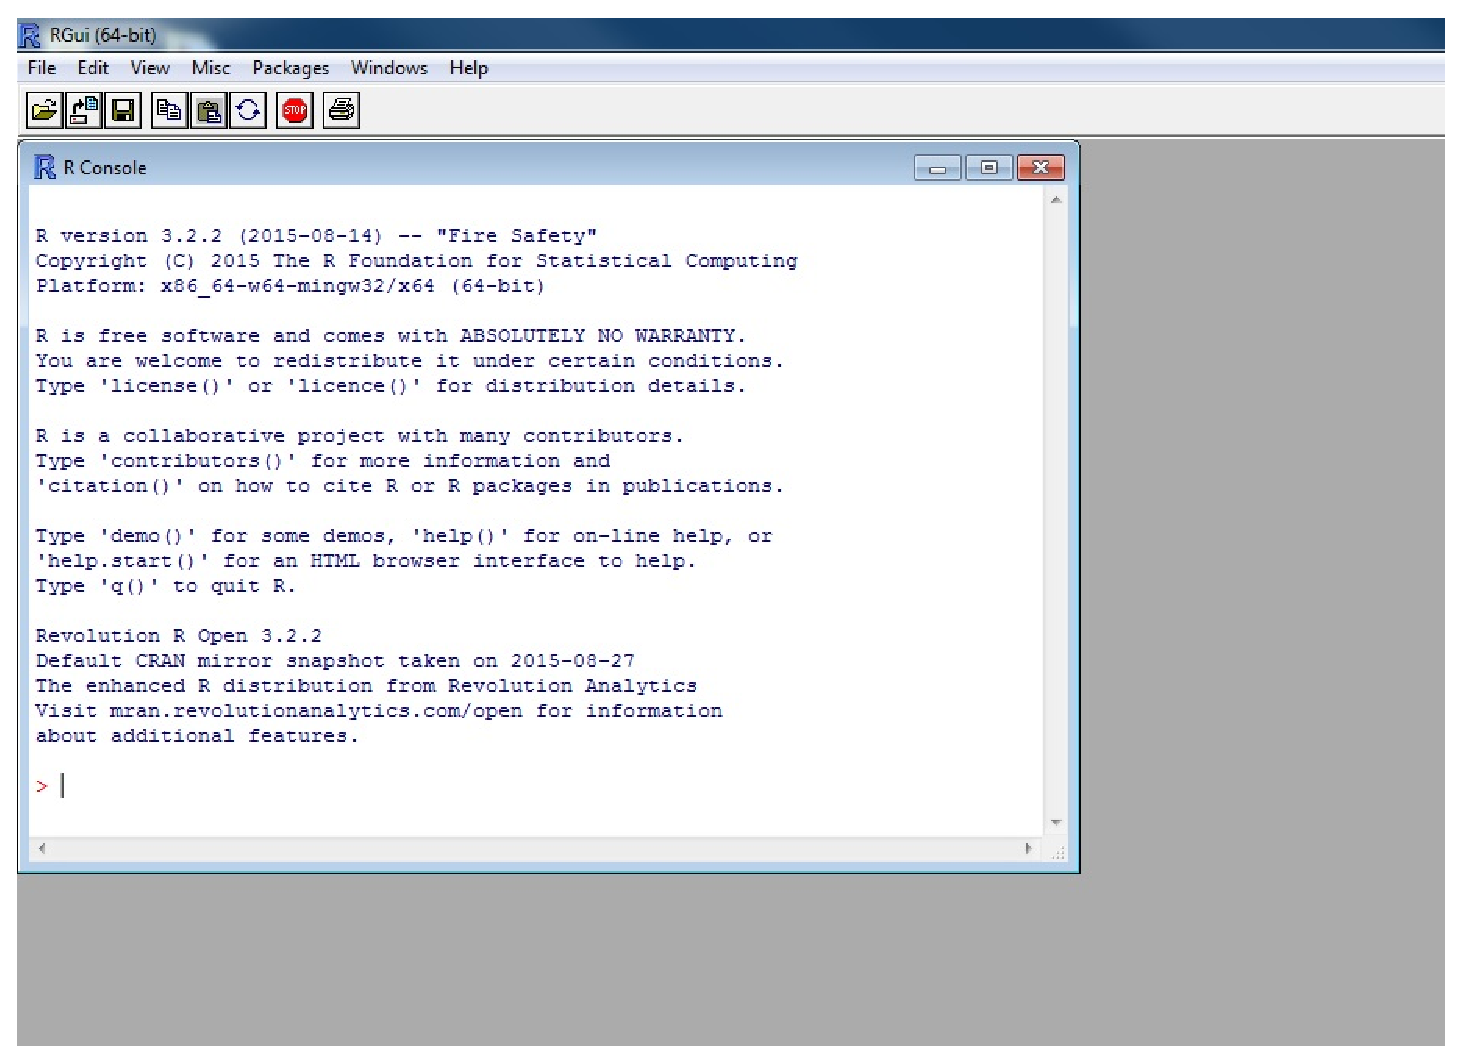
\includegraphics[height=0.6\textheight]{Figures/R.eps}  
\end{frame}
%======================================================
\begin{frame}[fragile]{Introduction (cont'd)}
\begin{itemize}
	\item What is \R ?
	\begin{itemize}
		\item is a software environment for statistical computing and graphics.
		\item Unlike SPSS, \R is purely command driven
	\end{itemize}
\end{itemize}
\end{frame}
%======================================================

\begin{frame}[fragile]{ Introduction (cont'd)}
\begin{itemize}
	\item Why \R ?
	\begin{itemize}
		\item R is a free software environment for statistical
		computing and graphics.
		\item it compiles and runs on LINUX, Windows and MacOS
		\item R has extensive and powerful graphics \& data manipulation
		capabilities
		\item it can easily interface with low-level programming
		languages, e.g., C/C++ or Fortran
		\item it can be easily extended via R packages
		\item the source code is available
		\item users are allowed to modify and redistribute the code
	\end{itemize}
\end{itemize}
\end{frame}
%======================================================
\begin{frame}[fragile]{ Introduction (cont'd)}
\begin{itemize}
	\item Where do I get \R ?
	\begin{itemize}
		\item \code{http://cran.r-project.org}
		\item choose your platform, e.g., Windows, Linux
		\item e.g., for Windows: \code{Windows} $\rightarrow$ \code{base}
		$\rightarrow$ \code{Download R 3.5.2 for Windows}
		\item Install $\ldots$
		\nl
	\end{itemize}
\end{itemize}
\end{frame}
%======================================================
\begin{frame}[fragile]{ Introduction (cont'd)}
\begin{itemize}
	\item How does \R work ?
	\begin{itemize}
		\item Packages built for specific tasks
		\item Download \R packages from the CRAN web site $\Rightarrow$ within \R
		\begin{itemize}
			\item[*] Packages
			\item[*] Install package(s) $\ldots$
			\item[*] make your choice(s)
			\item[*] load the package using \code{library()} (\textcolor{red}{note}:
			install does not mean load)
		\end{itemize}
	\end{itemize}
\end{itemize}
\end{frame}
%=====================================================
\begin{frame}{ Introduction (cont'd)}
\framesubtitle{How does \R work ?}
\vspace*{-3mm}
\includegraphics[height=0.7\textheight]{Figures/installpackages.eps}
\end{frame}
%======================================================
\begin{frame}{ Introduction (cont'd)}
\framesubtitle{How does \R work ?}
\vspace*{-3mm}
\includegraphics[height=0.7\textheight]{Figures/mean.eps}
\end{frame}
%======================================================
\begin{frame}{Introduction (cont'd)}
\framesubtitle{How to get help in \R }
%\vspace*{-2mm}
	\begin{itemize}
		\item Within R
		\begin{itemize}
			\item[*] \code{help.search("topic")} or \code{??"topic"} (depends on the
			installed packages)
			\item[*] \code{RSiteSearch("topic")} (requires internet connection)
			\item[*] \code{help()} or \code{?} invoke the on-line help file for the
			specified function
			\item[*] checking the FAQ
		\end{itemize}
	\end{itemize}
\end{frame}	
%======================================================
\begin{frame}{Introduction (cont'd)}
\framesubtitle{How to get help in \R }
	\begin{itemize}
		\item On the internet
		\begin{itemize}
			\item[*] \textsf{R}-help (\code{https://stat.ethz.ch/mailman/listinfo/r-help}
			-- mailing list)
			\item[*] \textsf{R}-seek (\code{http://www.rseek.org} -- Google-like
			searched engine)
			\item[*] \textsf{R}-wiki (\code{http://rwiki.sciviews.org/doku.php})
			\item[*] CRAN Task Views (\code{http://cran.r-project.org/web/views/}
			-- categorization of packages)	
		\end{itemize}
	\end{itemize}
\end{frame}
%======================================================
\begin{frame}[fragile]{Introduction (cont'd)}
\framesubtitle{How to get help in \R }
	\begin{itemize}
		\item On the internet
		\begin{itemize}
			\item[*] Crantastic (\code{http://crantastic.org/} -- categorization of
			packages $+$ reviews)
			\item[*] Equalis (\code{http://www.equalis.com/forums/} --
			\textsf{R} forum)
			\item[*] R4stats (\code{http://www.r4stats.com/} -- examples of basic \textsf{R} programs)
			\item[*] R related Blogs (\code{http://www.r-bloggers.com/} -- many useful illustrations of \textsf{R} and \textsf{R} packages)	
		\end{itemize}
\end{itemize}
\end{frame}
%======================================================
\begin{frame}[fragile]{ Introduction (cont'd)}
\framesubtitle{How to get help in \R }
\includegraphics[height=0.6\textheight]{Figures/help.eps}
\end{frame}
%======================================================
\begin{frame}[fragile]{ Introduction (cont'd)}
\framesubtitle{How to get help in \R }
\includegraphics[height=0.6\textheight]{Figures/help2.eps}
\end{frame}
%======================================================
\begin{frame}[fragile]{Introduction (cont'd)}
\framesubtitle{Disadvantages of \R}
\begin{itemize}
\item appears intimidating to the first-time user
\item output is not so nice looking (but there are some alternatives)
\item exporting output is more difficult
\end{itemize}
\end{frame}
%======================================================
\begin{frame}[fragile]{Introduction (cont'd)}
\framesubtitle{Disadvantages of \R}
\begin{itemize}
\item cannot easily handle very big data sets (depends on
the installed RAM)
\item a lot of things are available but it is sometimes hard to
find your way
\item the quality of the available packages is greatly varying
\end{itemize}
\end{frame}
%======================================================
\section{Part B}
%======================================================
\begin{frame}{1. Using \R}
\begin{itemize}
\item \R is a \textcolor{blue}{command}-based
\textcolor{red}{procedural} language
\begin{itemize}
\item write and execute \textcolor{blue}{commands}
\item use and define \textcolor{red}{functions}
\nl
\end{itemize}
\item You may write the commands in the R console (Windows)
or in a shell (Linux)
\nl
\nl
\nl
\begin{beamercolorbox}[wd=\linewidth, ht=2.5ex, dp=1.125ex,center]{palette secondary}
	\textbf{You will become more familiar with the syntax as you use it}
\end{beamercolorbox}
\end{itemize}
\end{frame}
%======================================================
\begin{frame}[fragile]{1. Using \R (cont'd)}
\begin{itemize}
	\item Strongly advisable to use a suitable text editor --
	Some available options:
	\begin{itemize}
		\item RWinEdt (for Windows; you also need WinEdt installed)
		\item Tinn-R (for Windows; \code{http://sciviews.org/Tinn-R/})
		\item Rkward (for Linux)
		\item Emacs (w. ESS, all platforms)
		\item Visual Studio (for Windows)
		\item Rstudio (all major platforms; \code{http://www.rstudio.org/})
		\item for more check
		\code{http://www.sciviews.org/\_rgui/projects/Editors.html}
	\end{itemize}
\end{itemize}
\end{frame}
%======================================================
\begin{frame}{1. Using \R (cont'd)}
\begin{itemize}
	\item For this course: \textcolor{red}{Rstudio} (\code{http://www.rstudio.org/})
	\begin{itemize}
		\item free
		\item works fine in Windows, MacOS and Linux
		\item helpful with errors
	\end{itemize}
\end{itemize}
\end{frame}
%======================================================
\begin{frame}{1. Using \R (cont'd)}
\begin{itemize}
\item Can I use R without Rstudio?
\item Can I use Rstudio without R?
\end{itemize}
\end{frame}
%======================================================
\begin{frame}{1. Using \R (cont'd)}
\begin{itemize}
\item R and Rstudio 
\newline\newline
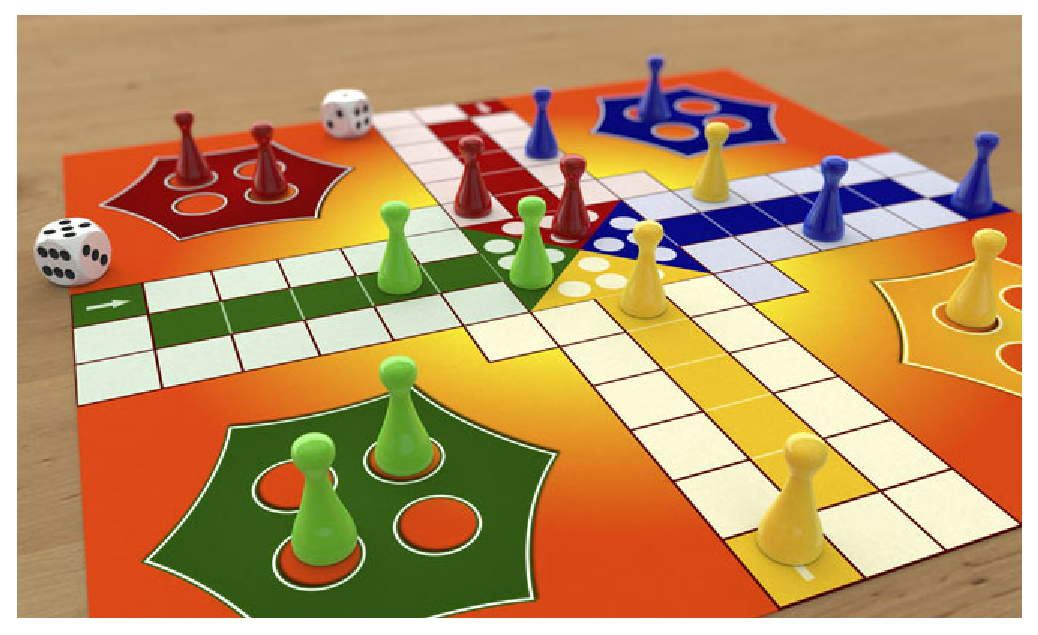
\includegraphics[width=0.4\textwidth, height=0.4\textheight]{Figures/BoardGame2.eps}   
\end{itemize}
\end{frame}
%======================================================
\begin{frame}{1. Using \R (cont'd)}
\begin{itemize}
\item R 
\newline\newline
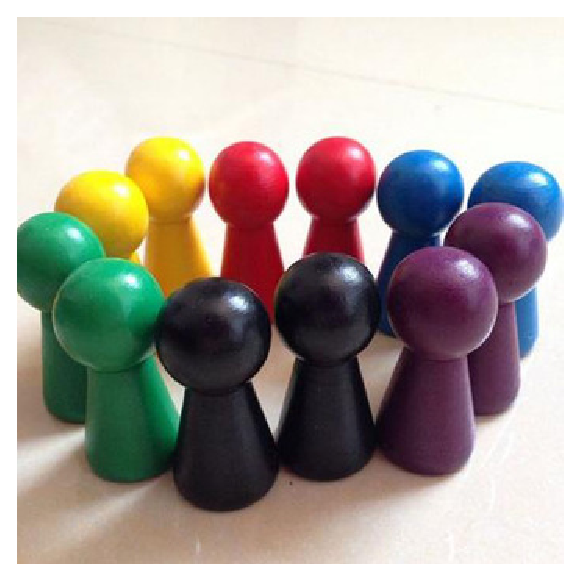
\includegraphics[width=0.3\textwidth, height=0.4\textheight]{Figures/BoardGame1.eps}   
\end{itemize}
\end{frame}
%======================================================
\begin{frame}{1. Using \R (cont'd)}
\begin{itemize}
\item Rstudio 
\newline\newline
\includegraphics[width=0.4\textwidth, height=0.4\textheight]{Figures/BoardGame3.eps}   
\end{itemize}
\end{frame}
%======================================================
 \begin{frame}[fragile]{2. Practical Examples}
\begin{tabular}{ccccccc}
	\textcolor{red}{id} &  \textcolor{red}{years} &  \textcolor{red}{status}  &  \textcolor{red}{drug} &  \textcolor{red}{age} & \dots &  \textcolor{red}{serBilir}\\
	1& 1.095170& dead&   D-penicil & 58.76684 & & 14.5\\
	2& 14.152338& alive&   D-penicil & 56.44782 & & 1.1\\
	3& 2.770781& dead& D-penicil & 70.07447 & & 1.4\\
	4& 5.270507& dead& D-penicil & 54.74209 & & 1.8\\
	5& 4.120578& transplanted&   placebo & 38.10645 & & 3.4\\                                                   
	6& 6.853028& dead&   placebo & 66.26054 & & 0.8\\
	\vdots &&&&&&
\end{tabular}
\end{frame}
%=====================================================
\begin{frame}[fragile]{2. Practical Examples (cont)}
\begin{itemize}
	\item What is a \textcolor{red}{dataset/vector}?
	\vspace{1ex}\vspace{1ex}
	\item Common \textcolor{red}{questions}
	\vspace{1ex}
	\begin{itemize}
		\item What is the \textcolor{blue}{average} age?
		\item What is the \textcolor{blue}{percentage} of drug?
		\item What is the \textcolor{blue}{average} age for \textcolor{blue}{males}?
		\item What is the \textcolor{blue}{average} age for \textcolor{blue}{drug}?
		\item What is the \textcolor{blue}{percentage} of alive people?
		\item \dots
	\end{itemize}
\end{itemize}
\end{frame}
%======================================================
\begin{frame}[fragile]{2. Practical Examples (cont)}
\begin{itemize}
\item \fbox{What is a \textcolor{red}{dataset/vector}?}
\end{itemize}
{\small\usebeamercolor[fg]{emcdblue}
	\begin{tabular}{ccccccc}
\textcolor{red}{id} &  \textcolor{red}{years} &  \textcolor{red}{status}  &  \textcolor{red}{drug} &  \textcolor{red}{age} & \dots &  \textcolor{red}{serBilir}\\
1& \textbf{1.095170}& dead&   D-penicil & 58.76684 & & 14.5\\
2& \textbf{14.152338}& alive&   D-penicil & 56.44782 & & 1.1\\
3& \textbf{2.770781}& dead& D-penicil & 70.07447 & & 1.4\\
4& \textbf{5.270507}& dead& D-penicil & 54.74209 & & 1.8\\
5& \textbf{4.120578}& transplanted&   placebo & 38.10645 & & 3.4\\                                                   
6& \textbf{6.853028}& dead&   placebo & 66.26054 & & 0.8\\
\vdots &&&&&&
\end{tabular}
}
\end{frame}
%======================================================
\begin{frame}{2. Practical Examples (cont)}
\begin{itemize}
\item Common \textcolor{red}{questions}
\vspace{1ex}
\begin{itemize}
\item \fbox{What is the \textcolor{blue}{average} age?}
\item \fbox{What is the \textcolor{blue}{percentage} of drug?}
\item What is the \textcolor{blue}{average} age for \textcolor{blue}{males}?
\item What is the \textcolor{blue}{average} age for \textcolor{blue}{drug}?
\item What is the \textcolor{blue}{percentage} of alive people?
\item \dots
\end{itemize}
\end{itemize}
\end{frame}

%======================================================
\begin{frame}[lbslide]{}
\begin{itemize}
\item \redbf{Let's go to the interactive tutorial!}
\end{itemize}
\end{frame}
%======================================================
\begin{frame}[fragile]{3. Basics in \R}
\begin{itemize}
	\item Elementary commands: \redbf{expressions} and
	\bluebf{assignments}
	\nl
	\item An \redbf{expression} given as command is evaluated printed
	and discarded
	\nl
	\item An \bluebf{assignment} evaluates an expression and passes the value to a
	variable -- the result is not automatically printed
\end{itemize}
\end{frame}

%======================================================
\begin{frame}[fragile]{3. Basics in \R (cont'd)}
\begin{itemize}
\item Expression is given as a command,
{\small
\begin{verbatim}
> 10
[1] 10
\end{verbatim}
}
\item However, it cannot be viewed again unless the command is rerun.
\item In order to store information, the expression should assign the command
{\small
\begin{verbatim}
> x <- 10
> x
[1] 10
\end{verbatim}
}
\end{itemize}
\end{frame}
%=================================================
\begin{frame}{3. Basics in \R (cont'd)}
\framesubtitle{Using R as a calculator}
\begin{itemize}
	\item Basic arithmetics
	\begin{itemize}
		\item \code{+}, \code{-}, \code{*}, \code{/}, \code{\^}
		\vspace{1ex}
		\vspace{1ex}
	\end{itemize}
	\item Complicated arithmetics
	\begin{itemize}
		\item \code{\%*\%}, \code{t()}, \code{\%/\%}
	\end{itemize}
\end{itemize}
\end{frame}
%======================================================
\begin{frame}[fragile]{3. Basics in \R (cont'd)}
\begin{itemize}
\item \R is case sensitive, e.g.,
\begin{itemize}
\item \code{"sex"} is different than \code{"Sex"}
\nl
\end{itemize}
\item Commands are separated by a semi-colon or by a newline
\nl
\item Comments can be put anywhere, starting with a hashmark (\#): everything to the end of the line is a comment
\nl
\item Assign a value to an object by $<$- or =
\end{itemize}
\end{frame}
%======================================================
\begin{frame}{3. Basics in \R (cont'd)}
\begin{itemize}
\item Missing values
\begin{itemize}
\item are coded as \code{NA} (i.e., not available) \code{is.na()}
\nl
\end{itemize}
\item Infinity
\begin{itemize}
\item is coded as \code{Inf} (plus infinity) or
\code{-Inf} (minus infinity) \code{is.finite()}
\nl
\end{itemize}
\item Not a number
\begin{itemize}
\item is coded as \code{NaN} (Not a Number) \\
Example: \code{0/0} \\
\code{[1] NaN}
\nl
\end{itemize}
\end{itemize}
\end{frame}
%======================================================
\begin{frame}[fragile]{4. Common \R Objects}
\vspace*{1mm}
{\small\usebeamercolor[fg]{emcdblue}
\begin{tabular}{cccccccc}
\textcolor{red}{id} &  \textcolor{red}{years} &  \textcolor{red}{status}  &  \textcolor{red}{drug} &  \textcolor{red}{age} & \dots &  \textcolor{red}{serBilir} & \textcolor{red}{age40higher}\\
1& 1.09517& dead&   D-penicil & 58.7668 & & 14.5 & TRUE\\
2& 14.15234& alive&   D-penicil & 56.4478 & & 1.1 & TRUE\\
3& 2.77078& dead& D-penicil & 70.0745 & & 1.4 & TRUE\\
4& 5.27051& dead& D-penicil & 54.7421 & & 1.8 & TRUE\\
5& 4.12058& transplanted&   placebo & 38.1065 & & 3.4 & FALSE\\                                                   
6& 6.853028& dead &   placebo & 66.2605 & & 0.8 & TRUE\\
\vdots &&&&&&&
\end{tabular}
}

\begin{beamercolorbox}[wd=\linewidth, ht=5ex, dp=1.125ex,center]{palette secondary}
 There are different kinds of variables.\\
  It depends on the type of variable what we can do with it
\end{beamercolorbox}
\end{frame}
%======================================================
%\begin{frame}[fragile]{4. Common \R Objects (cont'd)}
%\begin{itemize}
%\item Common \textcolor{red}{questions}
%\vspace{1ex}
%\begin{itemize}
%\item What is the \textcolor{blue}{average} age?
%\item What is the \textcolor{blue}{percentage} of drug?
%\item What is the \textcolor{blue}{average} age for \textcolor{blue}{males}?
%\item What is the \textcolor{blue}{average} age for \textcolor{blue}{drug}?
%\item \fbox{What is the \textcolor{blue}{percentage} of alive people?}
%\item \dots
%\end{itemize}
%\end{itemize}
%%======================================================
\begin{frame}[fragile]{4. Common \R Objects (cont'd)}
\begin{itemize}
\item in \R Everything (data, results, \ldots) is an object 
\item A variable is an object with a name so we can refer to it.
\item In order to list the created variables use \code{objects()} or \code{ls()}
{\small
\begin{verbatim}
> objects()
# Now remove all objects
> rm(list=ls(all=TRUE))
> objects()
character(0)
\end{verbatim}
}
\item To investigate a specific object \redbf{pbc2.id} use: \code{str(pbc2.id)}
\end{itemize}
\end{frame}
%======================================================
\begin{frame}[fragile]{4. Common \R Objects (cont'd)}
The simplest data structures are:
\begin{block}{Main types of \code{\textcolor{emclblue}{mode}}s}
  	\begin{itemize}
    \item \makebox[\widthof{\code{characterx}}][l]{\code{numeric}}: quantitative data
    \item \makebox[\widthof{\code{characterx}}][l]{\code{integer}}: whole numbers 
    \item \makebox[\widthof{\code{characterx}}][l]{\code{character}}: qualitative data
    \item \makebox[\widthof{\code{characterx}}][l]{\code{logical}}: TRUE or FALSE
    \item \makebox[\widthof{\code{characterx}}][l]{\code{raw}}: binary data - not discussed in this course 
    \item \makebox[\widthof{\code{characterx}}][l]{\code{complex}}: complex numbers $ai +b$ - not discussed
    \nl
  \end{itemize}
\end{block}   
\begin{itemize}
	\item Other data structures are composed of these \alert{atomic types}
  \item All atomic types are \alert{vectors}
 \end{itemize}
\end{frame}

\begin{frame}[fragile]{ 4. Common \R Objects (cont'd)}
  \begin{itemize}
    \item To find out what type of vector you have you can use the \alert{mode} function
    \item There are also other (non-atomic modes). We will discuss the most important ones (\code{list} and \code{function} later.)
  \end{itemize}
\end{frame}
%======================================================

\begin{frame}[fragile]{4. Common \R Objects (cont'd)}
\vspace*{-6mm}
\framesubtitle{Vectors}
{\small
	\begin{verbatim}
	> #Creating a vector consisting of 1,2, and 3
	> vector1 <- c(1,2,3)
	> vector1
	[1] 1 2 3
	> vector1 <- 1:3
	> vector1
	[1] 1 2 3
	\end{verbatim}
	\begin{verbatim}
	> #Creating a non-numeric vector
	> non.num.vector <- c("A","B","C")
	> non.num.vector
	[1] "A" "B" "C"
	\end{verbatim}
}
\end{frame}
%======================================================

\begin{frame}[fragile]{4. Common \R Objects (cont'd)}
\framesubtitle{Vectors}
\vspace*{-5mm}

% 	\item \R distinguishes between vectors, matrices, lists and dataframe %s
{\small
\begin{verbatim}
> # Running basic arithmetic operations
> vector1 + vector1
[1] 2 4 6
> # Initialize vector of size 3 and mode 'numeric'
> vector('numeric', 3)
\end{verbatim}
}


\end{frame}

\begin{frame}{4. Common \R Objects (cont'd)}
\begin{itemize}
\item Every object in \R has a \code{class}
\item This dictates how (some) generic methods (e.g., \code{print},
\code{summary}, etc.) deal with this object
\end{itemize}
\vspace*{-1mm}
Some common \R \code{\textcolor{emcdblue}{class}}es:
\vspace*{5mm}
\begin{tabular}{rcc}
\rowcolor{emcdblue}
	& \color{white}{Elements same type?} & \color{white}{Elements can be different} \\ 
\rowcolor{emclblue}	1d & \code{vector} & \code{list} \\ 
\rowcolor{emclblue}	2d & \code{matrix} & \code{data.frame} \\ 
\rowcolor{emclblue}	3d (or more) & \code{array} &  \\ 
\end{tabular} 
\end{frame}


%======================================================
\begin{frame}[fragile]{4. Common \R Objects (cont'd)}
\vspace*{-5mm}
\begin{itemize}
	\item \bluebf{Matrices} have the same type of elements
	\item \bluebf{Data.frames} and \bluebf{lists} do not need to have the same type of elements
	\item \bluebf{Lists} may have elements of different length
\end{itemize}
\end{frame}

%======================================================
\begin{frame}[fragile]{4. Common \R Objects (cont'd)}
\framesubtitle{Matrices and Arrays}
\vspace*{-5mm}
{\small
\begin{verbatim}
> matrix(vector2, 2, 2)
     [,1] [,2]
[1,]    1    3
[2,]    2    4
> matrix(vector2, 2, 2, byrow = TRUE)
     [,1] [,2]
[1,]    1    2
[2,]    3    4
> # create an array (output not shown)
> array(1:12,dim = c(3,2,4))  # 3 x 2 x 4 array (cube)
\end{verbatim}
}
\end{frame}
%======================================================


\begin{frame}[fragile]{4. Common \R Objects (cont'd)}
\framesubtitle{Lists}
\vspace*{-5mm}
{\small
	\begin{verbatim}
	> mylist = list(names = c("Jack","Mary"),
	child.ages = c(4,7,9,10,11))
	> mylist
	$names
	[1] "Jack" "Mary"
	$child.ages
	[1]  4  7  9 10 11
	> vector('list', 3) # initializes list (NB: not a vector)
	\end{verbatim}
}
\end{frame}
\begin{frame}[fragile]{4. Common \R Objects (cont'd)}
\vspace*{-5mm}
Differences between \bluebf{Matrices}, \bluebf{Data.frames} and \bluebf{lists}\newline\newline
\small{
\bluebf{Matrix}
$\begin{cases}
\begin{tabular}{cc}
\textcolor{red}{years} &  \textcolor{red}{age}  \\
1.095170& 58.76684\\
14.152338& 56.44782\\
2.770781& 70.07447\\
5.270507& 54.74209\\
4.120578& 38.10645\\
6.853028& 66.26054\\
\end{tabular}
\end{cases}$
}

%======================================================
\end{frame}
\begin{frame}[fragile]{4. Common \R Objects (cont'd)}
\vspace*{-5mm}
Differences between \bluebf{Matrices}, \bluebf{Data.frames} and \bluebf{lists}\newline\newline
\small{
\bluebf{Data frame}
$\begin{cases}
\begin{tabular}{ccccc}
\textcolor{red}{patient} &  \textcolor{red}{years} &  \textcolor{red}{age}  &  \textcolor{red}{sex} &  \textcolor{red}{age40higher} \\
1& 1.095170& 58.76684& female & TRUE\\
2& 14.152338& 56.44782& female & TRUE\\
3& 2.770781& 70.074473& male & TRUE\\
4& 5.270507& 54.74209& female & TRUE\\
5& 4.120578& 38.10645& female & FALSE\\
6& 6.853028& 66.26054& female & TRUE\\
\end{tabular}
\end{cases}$
}
%======================================================
\end{frame}
\begin{frame}[fragile]{4. Common \R Objects (cont'd)}
\vspace*{-5mm}
\only<1>{
Differences between \bluebf{Matrices}, \bluebf{Data.frames} and \bluebf{lists}\newline\newline
\small{
\bluebf{List}
$\begin{cases}
\begin{tabular}{cccc}
\textcolor{red}{years} &  \textcolor{red}{age}  &  \textcolor{red}{format}  &  \textcolor{red}{No patients per gender} \\
1.095170& 58.76684 & short format & females 88\\
14.152338& 56.44782 & & males 12\\
2.770781& 70.07447& &\\
5.270507& 54.74209& &\\
4.120578& 38.10645& &\\
6.853028& 66.26054& &\\
\end{tabular}
\end{cases}$
}}
\only<2>{
A \alert{factor} is a special kind of integer variable. Where each different value (called \alert{level}) has a \alert{label}. Used for categorical variables.\\
\code{factor(c(1, 2, 1), labels-=c('M', 'F')) )}



}
\end{frame}


%======================================================
\begin{frame}[fragile, t]{5. Importing Data and Saving your Work}
\vspace*{-5mm}
\begin{itemize}
\item \code{read.table()} and its variants
\begin{itemize}
\item \textcolor{red}{note}: use forward slashes or double backward slashes in the file names, e.g.,\\
\code{"C:/Documents and Settings/User/Data/file.txt"} or\\
\code{"C:\textbackslash\textbackslash Documents and Settings\textbackslash\textbackslash User\textbackslash\textbackslash Data\textbackslash\textbackslash file.txt"}
\nl
\end{itemize}
\item Specialized functions for importing data from other statistical packages
\begin{itemize}
\item packages \code{foreign},  \code{Hmisc} \& \code{readxl}
\item \code{read.spss()}, \code{read.csv()}, \code{read.dta()}, \code{sas.get()}, \code{read\_excel()}, etc.
\nl
\end{itemize}
\end{itemize}

\end{frame}

\begin{frame}[fragile]{5. Importing Data and Saving your Work}
\framesubtitle{Examples}
{\small
  \begin{verbatim}
  library(foreign)
  d1 <- read.spss("C:\\Documents and Settings\\User\\Data\\file.sav",
  to.data.frame=TRUE)
  
  d2 <- read.csv("C:\\Documents and Settings\\User\\Data\\file.csv") 
  \end{verbatim}
}
\end{frame}
%======================================================
\begin{frame}{5. Importing Data and Saving your Work (cont´d )}
\begin{itemize}
\item \code{ls()} lists \R objects in a session \& \code{rm()} removes objects
\nl
\item \code{save()}
\begin{itemize}
	\item can be used to save a list of \R objects
	\item a binary file with all the objects available in your last \R session
	\item platform independent
	\nl
\end{itemize}
\item You can load your saved \R objects using \code{load()}
\begin{itemize}
	\item be careful about overwriting
\end{itemize}
\item Using \code{saveRDS} and \code{readRDS} you can save and read a single \R object
\begin{itemize}
	\item The result has to be assigned to a variable
\end{itemize}
\end{itemize}
\end{frame}
%=================================================================


\begin{frame}[fragile]{5. Importing Data and Saving your Work (cont´d )}
\begin{itemize}
\item \redbf{To a TEXT file:}
\begin{verbatim}
write.csv(mydata, "c:/mydata.txt")
write.table(mydata, "c:/mydata.txt", sep="\t")
\end{verbatim}
\end{itemize}
\end{frame}
%======================================================

\begin{frame}[fragile]{5. Importing Data and saving your work (cont´d )}
\begin{itemize}
\item \redbf{To an Excel Spreadsheet:}
\begin{verbatim}
library(xlsx)
write.xlsx(mydata, "c:/mydata.xlsx")
\end{verbatim}
\end{itemize}
\end{frame}

\begin{frame}[fragile]{6. Data Transformation}
\begin{itemize}
	\item Round continuous variables
	\nl
	\item \code{numeric} variables to \code{factor}s
	\nl
	\item Compute new variables
	\begin{itemize}
		\item transform variables
		\nl
	\end{itemize}
	\item Matrices of \red{wide} $\Leftrightarrow$ \blue{long} format
	\nl
	\item Missing values and outliers
\end{itemize}
%======================================================
\end{frame}
\begin{frame}[fragile]{6. Data Transformation (cont'd)}
\begin{tabular}{ccccccc}
\textbf{id} &  \textbf{years} &  \textbf{status}  &  \textbf{drug} &  \textbf{age} & \dots &  \textbf{serBilir} \\
\textcolor{blue}{1}& \textcolor{blue}{1.10} & \textcolor{blue}{dead}&  \textcolor{blue}{ D-penicil} & \textcolor{blue}{58.77} & & \textcolor{blue}{14.5} \\
\textcolor{red}{2}& \textcolor{red}{14.15}& \textcolor{red}{alive}&   \textcolor{red}{D-penicil} & \textcolor{red}{56.45} & & \textcolor{red}{1.1}\\
3& 2.77& dead& D-penicil & 70.07 & & 1.4\\
4& 5.27& dead& D-penicil & 54.74 & & 1.8\\
5& 4.12& transplanted&   placebo & 38.11 & & 3.4\\                                                   
6& 6.85& dead&   placebo & 66.26 & & 0.8\\
\vdots &&&&&&
\end{tabular}
%======================================================
\end{frame}

\begin{frame}[fragile]{6. Data Transformation (cont'd)}
\begin{tabular}{ccccccc}
	\textbf{id} &  \textbf{years} &  \textbf{status}  &  \textbf{drug} &  \textbf{age} & \dots &  \textbf{serBilir} \\
	\textcolor{blue}{1}& \textcolor{blue}{1.10} & \textcolor{blue}{dead}&  \textcolor{blue}{ D-penicil} & \textcolor{blue}{58.77} & & \textcolor{blue}{14.5} \\
	\textcolor{blue}{1}& \textcolor{blue}{1.10} & \textcolor{blue}{dead}&  \textcolor{blue}{ D-penicil} & \textcolor{blue}{58.77} & & \textcolor{blue}{21.3} \\
	\textcolor{red}{2}& \textcolor{red}{14.15}& \textcolor{red}{alive}& \textcolor{red}{D-penicil} & \textcolor{red}{56.45} & & \textcolor{red}{1.1}\\
	\textcolor{red}{2}& \textcolor{red}{14.15}& \textcolor{red}{alive}& \textcolor{red}{D-penicil} & \textcolor{red}{56.45} & & \textcolor{red}{0.8}\\
	\textcolor{red}{2}& \textcolor{red}{14.15}& \textcolor{red}{alive}& \textcolor{red}{D-penicil} & \textcolor{red}{56.45} & & \textcolor{red}{1.0}\\
	\textcolor{red}{2}& \textcolor{red}{14.15}& \textcolor{red}{alive}& \textcolor{red}{D-penicil} & \textcolor{red}{56.45} & & \textcolor{red}{1.9}\\
	\vdots &&&&&&
\end{tabular}
%======================================================
\end{frame}
\begin{frame}[fragile]{7. Data Exploration}
\begin{itemize}
\item Common \textcolor{red}{questions}
\vspace{1ex}
\begin{itemize}
	\item \fbox{What is the \textcolor{blue}{mean} and \textcolor{blue}{sd} for age?}
	\item \fbox{What is the \textcolor{blue}{mean} and \textcolor{blue}{sd} for follow-up years?}
  \item What is the \textcolor{blue}{median} and \textcolor{blue}{interquartile range} for age?
 	\item What is the \textcolor{blue}{percentage} of drug and placebo?
	\item What is the \textcolor{blue}{mean} and \textcolor{blue}{sd} for age in \textcolor{blue}{males}?
  \item What is the \textcolor{blue}{mean} and \textcolor{blue}{sd} for follow-up years in \textcolor{blue}{females}?	
	\item What is the \textcolor{blue}{mean} and \textcolor{blue}{sd} for baseline serum bilirubin?
\end{itemize}
\end{itemize}

\end{frame}
%======================================================

\begin{frame}{7. Data Exploration (cont'd)}
\begin{itemize}
\item Common \textcolor{red}{questions}: \textbf{Hints}
\vspace{1ex}
\begin{itemize}
\item Check functions: \code{length(...)}, \code{mean(...)}, \code{min(...)}, \code{sd(...)}, \code{tapply(...)}, \code{median(...)}, \code{IQR(...)}, \code{quantile(...)}, \code{split}, \code{by} and \code{tapply}
\end{itemize}
\end{itemize}
%======================================================
\end{frame}

\begin{frame}[lbslide]{}
\begin{itemize}
	\item \redbf{Let's go to the interactive tutorial!}
\end{itemize}

%======================================================
\end{frame}


\begin{frame}{8. Indexing}
\vspace*{-0.5ex}
\begin{itemize}
	\item When transforming and analyzing data we often need to select specific observation or variables. 
	\nl
	\item\textbf{Examples}: Select \ldots
	\begin{itemize}
		\item \ldots the 3rd element for vector age
		\item \ldots the 3rd column of a matrix
		\item \ldots the sex of the 10th patient
        \item \ldots the baseline details of the 5th patient
        \item \ldots the serum cholesterol for all males
        \item \ldots the age for male patients or patients that have serum bilirubin more than 3
        \item \ldots first measurement per patient
	\end{itemize}
\end{itemize}
\end{frame}

\begin{frame}{8. Indexing (cont'd)}
\begin{itemize}
\item When transforming and analyzing data we often need to select specific observation or variables. 
\item This can be done using square bracket (\code{[},\code{]}) notation and \alert{indices}.
\nl
\item Three basic types
\begin{itemize}
	\item position indexing
	\item logical indexing
	\item name indexing
\end{itemize}
\end{itemize}
\end{frame}

\begin{frame}[fragile]{8. Indexing (cont'd)}
\framesubtitle{Position indexing with vectors}
\vspace*{-0.6ex}
{\small
\begin{verbatim}
  x <- c(5, 4, 7, 12, 2)	
\end{verbatim}
\vspace*{-0.3ex}	
\begin{itemize}
	\item Use \alert{positive value} to select an element. \code{x[2]} is \code{4}
	\item Multiple elements can be selected by using a (longer) vector of indices.\\ \code{x[c(2, 4])} is \code{c(4, 12)}
	\item Indices do not have to be in ascending order and may be duplicated.\\ \code{x[c(2, 2, 1)]} is \code{c(4, 4, 5)} 
	\item Use a \alert{negative index} to exclude elements. \code{x[c(-2, -4)]} is \code{c(5, 7, 2)}
	\item Positive and negative indices cannot be combined
\end{itemize}
}
\end{frame}

\begin{frame}[fragile]{8. Indexing (cont'd)}
\framesubtitle{Logical indexing with vectors}
\vspace*{-0.6ex}
{\small
	\begin{verbatim}
	  x <- c(5, 4, 7, 12, 2)	
	\end{verbatim}
}
	\vspace*{-0.3ex}	
	\begin{itemize}
		\item Use a logical index of the same length to select elements where the value is \code{TRUE}
	\end{itemize}
	\vspace*{-0.3ex}
\small{	
	\begin{verbatim}
      > i <- c(FALSE, TRUE, FALSE, TRUE, FALSE)
      > x[i]
      [1] 4 12	
    \end{verbatim}
}
\end{frame}

\begin{frame}[fragile]{8. Indexing (cont'd)}
\framesubtitle{Logical indexing with vectors}
\vspace*{-0.3ex}
{\small
\begin{verbatim}
x <- c(5, 4, 7, 12, 2)	
\end{verbatim}
}
\vspace*{-0.6ex}
	\begin{itemize}	
		\item Logical indexing is often used in combination with \textbf{conditions}
	\end{itemize}
\vspace*{-0.3ex}
{\small
	\begin{verbatim}
	> x[x > 5]
	[1] 4 7 12	
	\end{verbatim}
}
\end{frame}

\begin{frame}[fragile]{8. Indexing (cont'd)}
\framesubtitle{Name/ character indexing with vectors}
\vspace*{-1.2ex}
{\small
	\begin{verbatim}
	x <- c(foo=5, bar=4, one=7, two=12, three=2)	
	\end{verbatim}
\vspace*{-1ex}
\begin{itemize}	
	\item When a vector has been \textbf{named} the element names can be used as indices 
\end{itemize}
\vspace*{-1ex}
	\begin{verbatim}
	> x[c('foo', 'one')]
	foo one 
	5   7 	
	\end{verbatim}
\vspace*{-1ex}
\begin{itemize}	
	\item See the \code{names} function
	\item NB: A factor variable will not be converted to character when used as an index
\end{itemize}
}
\end{frame}

%======================================================

\begin{frame}[fragile]{8. Indexing (cont'd)}
\framesubtitle{Matrices and arrays}
\vspace*{-1ex}
\begin{itemize}
	\item Indexing matrices as similar to indexing vectors
	\item We now use a double index \code{x[i, j]} 
	\begin{itemize}
		\item[-] The first position denotes the \textbf{rows}
		\item[-] The first position denotes the \textbf{columns}
	\end{itemize}
    \item When we leave a position blank all elements are selected
   	\begin{itemize}
    	\item[-] e.g \code{M[c(2,3), ]} selects all columns of 2nd and 3rd row
    \end{itemize}
     \item When a single row or column is selected the matrix is converted to a vector unless \code{drop=FALSE} is used
     \item Indexing an array works the same way
\end{itemize}
\end{frame}

\begin{frame}[fragile]{8. Indexing (cont'd)}
\vspace*{-1ex}
\framesubtitle{Lists}
\begin{itemize}
	\item Lists can be subsetted in the same way as vectors using \code{[} and \code{]}, this always returns a list
	\item \textbf{Double square brackets} \code{[[} and \code{]]} can be used to extract a single element (what is in the list at this position)
    \item \code{\$} provides a convinient notation to extract an element by name  
\end{itemize}
\end{frame}

\begin{frame}[fragile]{8. Indexing (cont'd)}
\vspace*{-1ex}
\framesubtitle{Data.frames}
\begin{itemize}
	\item When you use a single index the data.frame acts like a \textbf{list of variables}
	\item When you using a double index, indexing works like a matrix
	\begin{itemize}
		\item The first position is used to select observations 
		\item The second position is used to select variables
	\end{itemize}
\end{itemize}
\end{frame}


%\begin{frame}[fragile]{8. Indexing (cont'd)}
%\begin{itemize}
%\item Indexing for vectors and matrices
%\nl
%\item Special indexing for \code{list}s and \code{data.frame}s
%\begin{itemize}
%\item the difference between \code{[}, \code{[[} and \code{\$}
%\item when should we use \code{drop = FALSE} for matrices and data frames
%\item indexing by row names (in \code{data.frame}s)
%\nl
%\end{itemize}
%\item Useful functions for indexing
%\begin{itemize}
%\item \code{match()}, \code{\%in\%}
%\item \code{rep()}, \code{seq()}
%\item \code{which()}, \code{which.min()}, \code{which.max()}
%\item \code{cut()}, \code{duplicated()}
%\end{itemize}
%\end{itemize}
%%======================================================
%\end{frame}

%======================================================

\begin{frame}[lbslide]{}
\begin{itemize}
\item \redbf{Let's go to the interactive tutorial!}
\end{itemize}

%======================================================
\end{frame}
\begin{frame}{9. Functions}
\begin{itemize}
\item What are functions \& how to define them
\begin{itemize}
\item each package has several functions
\item functions $\Rightarrow$ a group of (organized) \R commands
\nl
\end{itemize}
\item Why define functions?
\begin{itemize}
\item \R is a procedural language
\item Organize your code: easier to reuse, maintain and distribute to others
\item Formal definition of arguments
\item It protects from dangerous use of variable names
\nl
\end{itemize}
%\item Lexical scoping
\end{itemize}
%======================================================
\end{frame}

\begin{frame}{9. Functions (cont'd)}
\begin{itemize}
	\item How to use functions in packages
	\begin{itemize}
		\item study the on-line help file \code{(?mean)}, especially sections
		%\renewcommand{\labelitemi}{*}
		\begin{itemize}
			\item Arguments
			\item Value
			\item Examples
			\nl
		\end{itemize}
	\end{itemize}
\end{itemize}
\end{frame}
%===================================================
\begin{frame}{9. Functions (cont'd)}
\framesubtitle{Function parameters}
\begin{itemize}
  \item Most functions use \alert{parameters} (formal arguments)
  \item When you use them the parameters take the value of the arguments you provide in the function call
  \item You can specify the parameters by \textbf{name} \code{mean(x=x, na.rm=TRUE)} or \textbf{position} \code{mean(x, 0, TRUE)}
  \begin{itemize}
    \item First the parameter name is used then the arguments are matched by position
  \end{itemize} 
\item Often parameters have a \textbf{default value}
\end{itemize}
\end{frame}


\begin{frame}[fragile]{9. Functions (cont'd)}
\begin{itemize}
\item Some great and useful \R functions for \textcolor{red}{datasets}
\vspace{1ex}
\vspace{1ex}
\begin{itemize}
	\item What is the number of males and females? \code{table()}
	\item What is the mean weight and height? \code{mean()}, 
	\item How many patients are included in the dataset? \code{length()}
	\item Divide the dataset into groups. \code{split()}
\end{itemize}
\end{itemize}
%======================================================
\end{frame}
\begin{frame}[fragile]{9. Functions (cont'd)}
\begin{itemize}
\item Some great and useful \R functions for \textcolor{red}{vectors} in general
\vspace{1ex}
\vspace{1ex}
\begin{itemize}
\item Create a sequence. \code{seq()}
\item Create a vector with repeated values. \code{rep()}
\item Obtain all possible combinations. \code{expand.grid()}
\item Combine vectors by columns or rows. \code{cbind()}, \code{rbind()}
\end{itemize}
\end{itemize}
%======================================================
\end{frame}
\begin{frame}[label=functions]{9. Functions (cont'd)}
\begin{block}{You can also create your own functions!}
\begin{itemize}
\item Easily use the code again for different data
\item Distribute to others
\end{itemize}
\end{block}
% \hyperlink{ownfunctions}{\beamerbutton{show me}}.
\end{frame}

\begin{frame}[fragile, label=ownfunctions]{9. Functions (cont'd)}
Define function:\\
{\small
\begin{Verbatim}[commandchars=\\\[\]]
myfunction <- function(arg1, opt2=2, ...){

 \fbox[\blue[functionbody] ]

 return(...)
}
\end{Verbatim}
}
Use the function:
{\small
\begin{verbatim}
myfunction(1, 2)  myfunction(1, opt2=2)  myfunction(1) 
\end{verbatim}
}
% Back to \hyperlink{functions}{\beamerbutton{functions}}.
\end{frame}
%======================================================


\begin{frame}{9. Functions (cont'd)}
\begin{itemize}
  \item When your function gives you an error it can be usefull to use the \code{debug} function to find it
  \item If your function works correctly but you want to improve it's speed you can use the \code{microbenchmark} package.
\end{itemize}
\end{frame}


\begin{frame}{10. Loops and Control Flow}
\begin{itemize}
	\item Loops:
	\begin{itemize}
		\item \textcolor{red}{Repeat a statistical test or a computation}
		\begin{itemize}
			\item[-] \code{for()}: loop over a sequence of values, e.g., iterations
			\item[-] \code{while()}: loop as long as a prespecified condition is satisfied
			\item[-] \code{replicate()}: replicate a number of times
		\end{itemize}
	\end{itemize}
	\item Control flow:
	\begin{itemize}
		\item \textcolor{red}{Perform a statistical test or a computation in specific cases}
		\begin{itemize}
			\item[-] \code{if}-\code{else}: standard control flow
			\item[-] \code{ifelse()}: conditional element selection (vectorized version)
			\item[-] \code{switch()}: select one of a list of alternatives
		\end{itemize}
	\end{itemize}
\end{itemize}
%======================================================
\end{frame}
\begin{frame}[fragile]{10. Loops and Control Flow (cont'd)}
\vspace*{-5mm}
{\small
\begin{verbatim}
> for (i in 1:10){ print(i) }
[1] 1
[1] 2
[1] 3
[1] 4
[1] 5
[1] 6
[1] 7
[1] 8
[1] 9
[1] 10
\end{verbatim}
}
%======================================================
\end{frame}
\begin{frame}[fragile]{10. Loops and Control Flow (cont'd)}
\begin{verbatim}
> for (i in 1:10){
if (i < 5) {
print(i)
}
}
[1] 1
[1] 2
[1] 3
[1] 4
\end{verbatim}


%======================================================
\end{frame}
\begin{frame}[fragile]{11. The apply Family}
\begin{itemize}
\item Manipulate slices of data from matrices, arrays, lists and dataframes in a repetitive way avoiding explicit use of loop constructs
\nl
\begin{itemize}
\item An aggregating function, like for example the mean, or the sum 
\item Other transforming or subsetting functions
\item Other vectorized functions, which return more complex structures like lists, vectors, matrices and arrays
\end{itemize}
\end{itemize}

%======================================================
\end{frame}


\begin{frame}[fragile]{11. The apply Family  (cont'd)}
\begin{verbatim}
apply(), lapply() , sapply(), tapply(), mapply()
\end{verbatim}
\textbf{But how and when should we use these?}

%======================================================
\end{frame}
\begin{frame}[fragile]{11. The apply Family  (cont'd)}
\redbf{How To Use apply() in R}
\nl
\begin{itemize}
\item operates on arrays/matrices
\end{itemize}
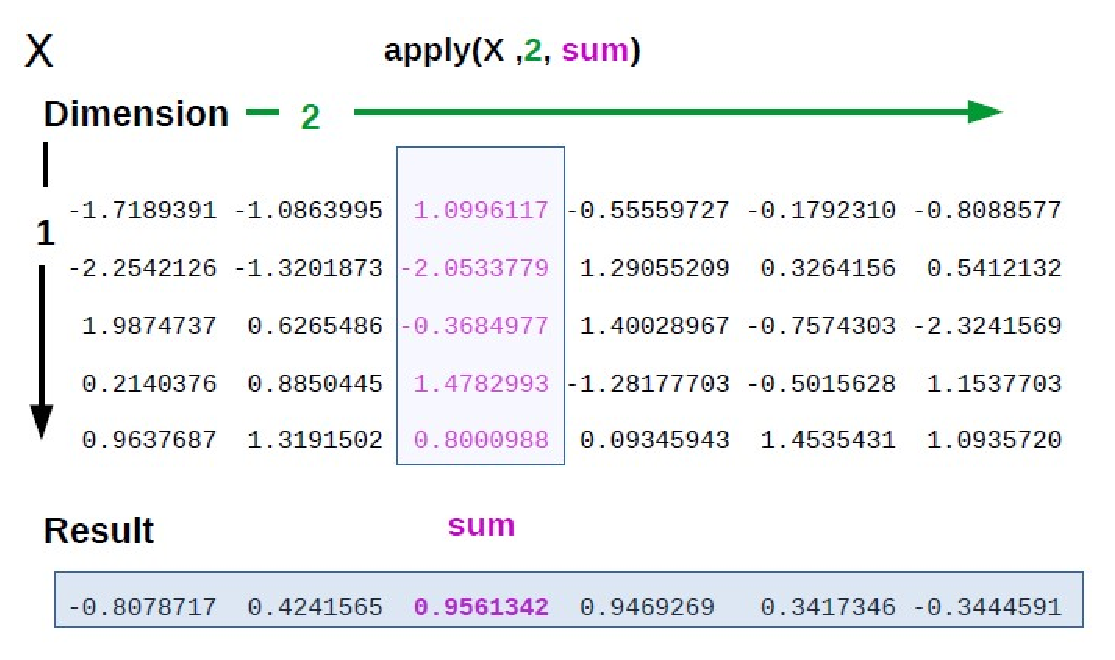
\includegraphics[scale=0.4]{Figures/apply.eps}

%======================================================
\end{frame}
\begin{frame}[fragile]{11. The apply Family  (cont'd)}
\redbf{How To Use lapply() in R}
\begin{itemize}
\item You want to apply a given function to every element of a list and obtain a list as result
\item The difference with apply():
\nl
\begin{itemize}
\item It can be used for other objects like dataframes, lists or vectors
\item The output returned is a list
\end{itemize}
\end{itemize}
%======================================================
\end{frame}
\begin{frame}[fragile]{11. The apply Family  (cont'd)}
\redbf{How To Use sapply() in R}
\begin{itemize}
\item sapply() is similar to lapply(), but it tries to simplify the output 
\end{itemize}
%======================================================
\end{frame}
\begin{frame}[fragile]{11. The apply Family  (cont'd)}
\redbf{How To Use tapply() in R}
\begin{itemize}
\item Apply a function to subsets of a vector and the subsets are defined by some other vector, usually a factor
\end{itemize}
%======================================================
\end{frame}
\begin{frame}[fragile]{11. The apply Family  (cont'd)}
\redbf{How To Use mapply() in R}
\begin{itemize}
\item Multivariate apply
\item Its purpose is to be able to vectorize arguments to a function that is not usually accepting vectors as arguments
\item mapply() applies a function to multiple list or multiple vector arguments.
\end{itemize}

%======================================================
\end{frame}
\begin{frame}[fragile]{12. Merging Data Sets}
\begin{itemize}
	\begin{small}
\item \redbf{EXAMPLE 1}: (basic)

\item \redbf{EXAMPLE 2}: in one dataset a subcategory is missing from a variable

\item \redbf{EXAMPLE 3}: merge many rows to one

\item \redbf{EXAMPLE 4}: common IDs have different variable name in the 2 data sets

\item \redbf{EXAMPLE 5}: different data set variables but same variable name
\nl
    \end{small}
\end{itemize}
\centering
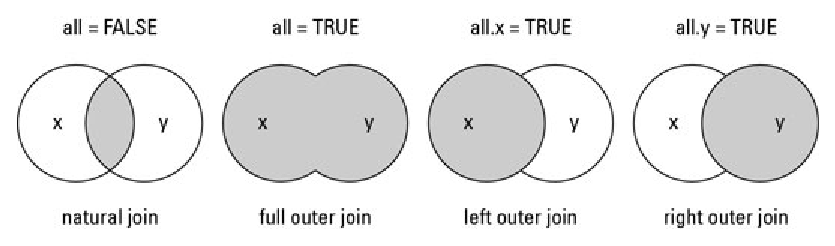
\includegraphics[scale=0.75]{Figures/merge.eps}
%======================================================
\end{frame}

\begin{frame}[lbslide]{}
\begin{itemize}
	\item \redbf{Let's go to the interactive tutorial!}
\end{itemize}
\end{frame}



\begin{frame}[fragile]{13 Graphs}
\begin{itemize}
\item \R has very powerful graphics capabilities
\nl
\item Some good references are
\begin{itemize}
  \item Murrel, P. (2005) \emph{R Graphics}. Boca Raton: Chapman \& Hall/CRC.
  \item Sarkar, D. (2008) \emph{Lattice Multivariate Data Visualization with R}. New York: Springer-Verlag.
  \nl
\end{itemize}
\end{itemize}
%======================================================
\end{frame}
\begin{frame}{13 Graphs (cont'd)}
\begin{itemize}
\item Traditional graphics system
\begin{itemize}
\item package \code{graphics}
\nl
\end{itemize}
\item Trellis graphics system
\begin{itemize}
\item package \code{lattice} (which is based on package \code{grid})
\nl
\end{itemize}
\item Grammar of Graphics implementation (i.e., Wilkinson, L. (1999) \emph{The Grammar of Graphics}. New York: Springer-Verlag)
\begin{itemize}
\item packages \code{ggplot} \& \code{ggplot2}
\end{itemize}
\end{itemize}
\end{frame}
%======================================================

 \begin{frame}[fragile]{13. Graphs}
\begin{itemize}
	\item Important plotting functions
	\begin{itemize}
		\item \code{plot()}: scatter plot (and others)
		\item \code{barplot()}: bar plots
		\item \code{boxplot()}: box-and-whisker plots
		\item \code{dotchart()}: dot plots
		\item \code{hist()}: histograms
		\item \code{pie()}: pie charts
		\item \code{qqnorm()}, \code{qqline()}, \code{qqplot()}:  distribution plots
		\item \code{pairs()}: for multivariate data
	\end{itemize}
\end{itemize}
%%======================================================
\end{frame}
  \begin{frame}[fragile]{13. Graphs (cont'd)}
\begin{itemize}
	\item Controlling the appearance of plots
	\begin{itemize}
		\item position of the plots
		\item graphical parameters
	\end{itemize}
\end{itemize}
%======================================================
\end{frame}
\begin{frame}[fragile]{14. Statistical Tests}
\begin{tabular}{ccccccc}
\textcolor{red}{id} &  \textcolor{red}{years} &  \textcolor{red}{status}  &  \textcolor{red}{drug} &  \textcolor{red}{age} & \dots &  \textcolor{red}{serBilir}\\
1& 1.095170& dead&   D-penicil & 58.76684 & & 14.5\\
2& 14.152338& alive&   D-penicil & 56.44782 & & 1.1\\
3& 2.770781& dead& D-penicil & 70.07447 & & 1.4\\
4& 5.270507& dead& D-penicil & 54.74209 & & 1.8\\
5& 4.120578& transplanted&   placebo & 38.10645 & & 3.4\\                                                   
6& 6.853028& dead&   placebo & 66.26054 & & 0.8\\
\vdots &&&&&&
\end{tabular}
%======================================================
\end{frame}
\begin{frame}[fragile]{14. Statistical Tests  (cont'd)}
\begin{itemize}
\item \textcolor{red}{Is there a difference in serum bilirubin values between drug and placebo?}
\begin{itemize}
\item \textcolor{blue}{T-test}
\begin{itemize}
	\item[-] null hypothesis $H_0 : \mu_1 = \mu_2$ (the population means in the two groups are equal)
	\item[-] assumption: data is approximately normally distributed or large enough sample
\end{itemize}
\end{itemize}
\item \textcolor{red}{Is there a difference in age between the status groups?}
\begin{itemize}
\item \textcolor{blue}{Anova}
\begin{itemize}
	\item[-] extension of tests for testing two means, now testing two or more groups
	\item[-] null hypothesis $H_0 : \mu_1 = \mu_2 = \mu_3 = \dots$
\end{itemize}
\end{itemize}
\end{itemize}
%======================================================
\end{frame}
\begin{frame}[fragile]{14. Statistical Tests (cont'd)}
\begin{itemize}
\item \textcolor{red}{Is there a difference in serum bilirubin values between drug and placebo?}
\begin{itemize}
\item \textcolor{blue}{Wilcoxon test} -  Nonparametric alternative
\begin{itemize}
\item[-] Based on the sum of the ranks of the values in both groups
\item[-] Unlike the t-test it does not require the assumption of normal distributions
\item[-] $H_0$: samples from the two groups come from the same distribution
\end{itemize}
\end{itemize}
\item \textcolor{red}{Is there a difference in age between the status groups?}
\begin{itemize}
\item \textcolor{blue}{Kruskal-Wallis test} -  Nonparametric alternative
\begin{itemize}
\item[-] Applied if equality of variances does not hold
\item[-] It is an extension of the Wilcoxon rank sum test to 3 or more groups
\item[-] $H_0$: each group has the same distribution of values in the population
\end{itemize}
\end{itemize}
\end{itemize}
%======================================================
\end{frame}
\begin{frame}[fragile]{14. Statistical Tests (cont'd)}
\begin{itemize}
\item \textcolor{red}{Are the variables status and drug independent?}
\begin{itemize}
\item \textcolor{blue}{Chi-square test}
\begin{itemize}
\item[-] $H_0$: 2 categorical variables are independent
\item[-] Chi-square should not be calculated if the expected value in any category is $<$ 5
\vspace{1ex}
\vspace{1ex}
\end{itemize}
\item \textcolor{blue}{Fisher's exact test} 
\begin{itemize}
\item[-] Nonparametric alternative
\end{itemize}
\end{itemize}
\end{itemize}
%======================================================
\end{frame}
\begin{frame}[fragile]{14. Statistical Tests (cont'd)}
\begin{itemize}
\item \textcolor{red}{Is there a linear association between age and serum bilirubin?}
\begin{itemize}
\item \textcolor{blue}{Correlations} - \textbf{Pearson}, \textbf{Spearman}
\vspace{1ex}
\vspace{1ex}
\begin{itemize}
\item \makebox[\widthof{\code{character}}][l]{$r = 0$}, no linear correlation
\item \makebox[\widthof{\code{character}}][l]{$r > 0$}, positive linear correlation
\item \makebox[\widthof{\code{character}}][l]{$r < 0$}, negative linear correlation
\item \makebox[\widthof{\code{character}}][l]{$r = 1$}, perfect positive linear correlation
\item \makebox[\widthof{\code{character}}][l]{$r = -1$}, perfect negative linear correlation
\end{itemize}
\end{itemize}
\end{itemize}
%======================================================
\end{frame}
\begin{frame}[fragile]{14. Statistical Tests (cont'd)}
\begin{itemize}
\item In some cases, extreme values may be obtained
\vspace{1ex}
\vspace{1ex}
\item Most of the times we exclude the outliers
\end{itemize}
%======================================================
\end{frame}
\begin{frame}[fragile]{15. Regression Models}
\begin{itemize}
\item What it the association of \redbf{age} with \redbf{serum bilirubin} accounting for \redbf{sex} and \redbf{drug}?
\begin{itemize}
\item Linear regression models
\begin{itemize}
\item[-] response variable $y$ continuous
\item[-] covariates $x_1, x_2, \dots$
\item[-] $H_0$: $\beta$ is zero
\item[-] assumption: errors are approximately normally distributed
\item[-] model: $y = \beta_0 + \beta_1x_1 + \beta_2x_2 + \dots + \dots + \beta_kx_k + \epsilon$, $\epsilon \sim N(0,\sigma^2)$
\vspace{1ex}
\end{itemize}
\item In R using \code{lm()}
\begin{itemize}
\item[-] different options for the \code{formula} argument
\item[-] summarizing the fitted models: hypothesis testing, plots, etc.
\nl
\end{itemize}
\end{itemize}
\end{itemize}
%======================================================
\end{frame}
\begin{frame}[fragile]{15. Regression Models (cont'd)}
\begin{itemize}
\item What it the association of \redbf{age} with \redbf{drug} accounting for \redbf{sex}?
\begin{itemize}
\item Logistic regression models
\begin{itemize}
\item[-] response variable $y$ dichotomous
\item[-] covariates $x_1, x_2, \dots$
\item[-] $H_0$: $\beta$ is zero
\item[-] model: $\ln(\frac{y}{1-y}) = \beta_0 + \beta_1x_1 + \beta_2x_2 + \dots + \dots + \beta_kx_k$
\vspace{1ex}
\end{itemize}
\item In R using \code{glm()}
\begin{itemize}
\item[-] different options for the \code{family} argument
\end{itemize}
\end{itemize}
\end{itemize}
%======================================================
\end{frame}
\begin{frame}[fragile]{15. Regression Models (cont'd)}
\begin{itemize}
\item Using formulas in \R
\begin{itemize}
\item serBilir = age + sex + drug \nl$\Rightarrow$ \fbox{\code{serBilir $\sim$ age + sex + drug}}
\nl
\item serBilir = age + sex + drug + age*sex \nl$\Rightarrow$ \fbox{\code{serBilir $\sim$ age + sex + drug + age:sex}}\nl
$\Rightarrow$ \fbox{\code{serBilir $\sim$ drug + age*sex}} (the same)
\nl
\item serBilir = age + age$^2$ \nl$\Rightarrow$ \fbox{\code{serBilir $\sim$ age + I(age\textasciicircum 2)}}
\nl
\item drug = age + sex \nl$\Rightarrow$ \fbox{\code{drug $\sim$ age + sex}}
\nl
\end{itemize}
\end{itemize}
\end{frame}
%======================================================
\begin{frame}[fragile]{15. Regression Models (cont'd)}
\begin{itemize}
	\item Formulas are used to define statistical regression models in \R but also in
	other functions to denote a relationship between a response variable and covariates
	\nl
	\item A lot of other statistical modeling techniques are available via \R packages
	\nl
	\item The basic structure is:\\\hspace{2cm}
	\code{model.function(formula, data, ...)}
\end{itemize}
\end{frame}
%======================================================
\begin{frame}[lbslide]{}
\begin{itemize}
	\item \redbf{Let's go to the interactive tutorial!}
\end{itemize}
\end{frame}
%======================================================
\begin{frame}{Review of Key Points}
\begin{itemize}
\item The \code{str()} function can be used to compactly display the structure of an \R object
\nl
\item Data manipulations
\begin{itemize}
\item use indexing
\item some useful functions \code{split()}, \code{ave()}, \code{table()}, \code{duplicated()}, \dots
\end{itemize}
\end{itemize}
\end{frame}
%======================================================
\begin{frame}{Review of Key Points (cont'd)}
\begin{itemize}
\item Functions
\begin{itemize}
\item split big calculations in smaller steps
\item make your code easier to read and maintain
\nl
\end{itemize}
\item Graphs
\begin{itemize}
\item for standard plots use \code{plot()}, $\ldots$
\item for conditioning plots \code{xyplot()}, $\ldots$
\end{itemize}
\end{itemize}
\end{frame}
%======================================================
\begin{frame}[fragile]{Review of Key Points (cont'd)}
\begin{itemize}
	\item Formulas are used to define statistical regression models in \R but also in
	other functions to denote a relationship between a response variable and covariates
	\nl
	\item A lot of other statistical modeling techniques are available via \R packages
	\nl
	\item The basic structure is:\\\hspace{2cm}
	\code{model.function(formula, data, ...)}
\end{itemize}
\end{frame}
%======================================================
\begin{frame}{Review of Key Points (cont'd)}
\begin{itemize}
\item \code{ls()} lists \R objects in a session \& \code{rm()} removes objects
\nl
\item \code{save()}
\begin{itemize}
	\item can be used to save a list of \R objects
	\item a binary file with all the objects available in your last \R session
	\item platform independent
	\nl
\end{itemize}
\item You can load your saved \R objects using \code{load()}
\begin{itemize}
	\item be careful about overwriting
\end{itemize}
\end{itemize}
\end{frame}
%======================================================
  \begin{frame}[fragile]{Review of Key Points (cont'd)}
\fbox{\redbf{\R can do everything \dots we just need to figure out how \dots}}
\end{frame}
%======================================================
%======================================================
%======================================================
%======================================================
\section{Part C}
%======================================================

\begin{frame}[fragile]{1. Markdown}
\begin{itemize}
\item R Markdown is a format for writing \alert{reproducible, dynamic reports} with R
\item Use it to \alert{embed R code and results} into slideshows, pdfs, html documents, Word files and more
\end{itemize}
\end{frame}
\begin{frame}[fragile]{1. Markdown (cont'd)}
\begin{itemize}
\item In \redbf{Rstudio}
\vspace{1ex}
\vspace{1ex}
\begin{itemize}
\item File $\rightarrow$ New File $\rightarrow$ R Markdown...
\item Insert title and author
\item Select format
\end{itemize}
\end{itemize}
\end{frame}



%======================================================
\begin{frame}[fragile, t]{1. Markdown (cont'd)}
\begin{itemize}
	\item \redbf{Writing-part}
	\begin{itemize}
		\item[] \fbox{Header}
		
		\begin{columns}
			\begin{column}{0.45\textwidth}
				\vspace{1cm}
				\begin{itemize}
					\item Input
					
					\begin{code11}
						# Methods
						## Data collection
						## Statistical analysis
						# Results
					\end{code11}
				\end{itemize}
				
			\end{column}%
			\hfill
			\begin{column}{0.45\textwidth}
				\vspace{1cm}
				\begin{itemize}
					\item Output
					
					\large{Methods}
					\\
					\normalsize{Data collection}
					\\
					\normalsize{Statistical analysis}
					\\
					\large{Results}  
				\end{itemize}
				
			\end{column}%
		\end{columns}
	\end{itemize}
\end{itemize}
\end{frame}

\begin{frame}[fragile, t]{1. Markdown (cont'd)}
\begin{itemize}
	\item \redbf{Writing-part}
	\begin{itemize}
		\item[] \fbox{Emphasis}
		
		
		\begin{columns}
			\begin{column}{0.45\textwidth}
				\vspace{1cm}
				\begin{itemize}
					\item Input
					
					\begin{code11}
						*Methods*  
						_Methods_
						**Methods**
						__Methods__
					\end{code11}
				\end{itemize}
			\end{column}%
			\hfill
			\begin{column}{0.45\textwidth}
				\vspace{1cm}
				\begin{itemize}
					\item Output
					
					\textit{Methods}
					\\
					\textit{Methods}
					\\
					\textbf{Methods}
					\\
					\textbf{Methods}
					\\  
				\end{itemize}
			\end{column}%
		\end{columns}
	\end{itemize}
\end{itemize}

%======================================================
\end{frame}
\begin{frame}[fragile, t]{1. Markdown (cont'd)}
\begin{itemize}
\item \redbf{Writing-part}
\begin{itemize}
	\item[] \fbox{Bullets}
	
	\begin{columns}
		\begin{column}{0.45\textwidth}
			\vspace{1cm}
			\begin{itemize}
				\item Input
				
				\begin{code11}
					* Method 1
					- Method 2
					+ Method 3
				\end{code11}
			\end{itemize}
		\end{column}%
		\hfill
		\begin{column}{0.45\textwidth}
			\vspace{1cm}
			\begin{itemize}
				\item Output
				
				$\bullet$ Method 1
				\\
				$\bullet$ Method 2
				\\
				$\bullet$ Method 3
				\\  
			\end{itemize}
		\end{column}%
	\end{columns}%
\end{itemize}
\end{itemize}




%======================================================
\end{frame}
\begin{frame}[fragile, t]{1. Markdown (cont'd)}
\begin{itemize}
\item \redbf{Writing-part}
\begin{itemize}
\item[] \fbox{Bullets}


\begin{columns}
	\begin{column}{0.45\textwidth}
		\vspace{1cm}
		\begin{itemize}
			\item Input
			
			\begin{code11}
				* Method 1
				- Method 2
				    + Method 3
			\end{code11}
		\end{itemize}
	\end{column}%
	\hfill
	\begin{column}{0.45\textwidth}
		\vspace{1cm}
		\begin{itemize}
			\item Output
			
			$\bullet$ Method 1
			\\
			$\bullet$ Method 2
			
			\hspace{0.6cm} $\circ$  Method 3
			
			
		\end{itemize}
	\end{column}%
\end{columns}%
\end{itemize}
\end{itemize}


%======================================================
\end{frame}
\begin{frame}[fragile, t]{1. Markdown (cont'd)}
\begin{itemize}
\item \redbf{Writing-part}
\begin{itemize}
\item[] \fbox{Links}

\begin{columns}
\begin{column}{0.45\textwidth}
	\vspace{1cm}
	\begin{itemize}
		\item Input
		
		\begin{code11}
			[link](http://example.com)
		\end{code11}
	\end{itemize}
\end{column}%
\hfill
\begin{column}{0.45\textwidth}
	\vspace{1cm}
	\begin{itemize}
		\item Output
		\\
		\underline{\blue{link}}
		
	\end{itemize}
\end{column}%
\end{columns}%
\end{itemize}
\end{itemize}




%======================================================
\end{frame}
\begin{frame}[fragile, t]{1. Markdown (cont'd)}
\begin{itemize}
\item \redbf{Writing-part}
\begin{itemize}
\item[] \fbox{Images}

\begin{columns}
\begin{column}{0.45\textwidth}
\vspace{1cm}
\begin{itemize}
	\item Input
	
	\begin{code11}
		![Rsymbol](https://
		upload.wikimedia.org/
		wikipedia/commons/1/12/
		R_logo_2000.png)
	\end{code11}
\end{itemize}
\end{column}%
\hfill
\begin{column}{0.45\textwidth}
\vspace{0cm}
\begin{itemize}
	\item Output
	\\
	\bluebf{Guess???}
	
\end{itemize}
\end{column}%
\end{columns}
\end{itemize}
\end{itemize}



%======================================================
\end{frame}
\begin{frame}[fragile, t]{1. Markdown (cont'd)}
\begin{itemize}
\item \redbf{Writing-part}
\begin{itemize}
\item[] \fbox{Images}

\begin{columns}
\begin{column}{0.45\textwidth}
\vspace{1cm}
\begin{itemize}
\item Input

\begin{code11}
	![Rsymbol](https://
	upload.wikimedia.org/
	wikipedia/commons/1/12/
	R_logo_2000.png)
	{ width=50% }
	\end{code11}
\end{itemize}
\end{column}%
\hfill
\begin{column}{0.45\textwidth}
\vspace{0cm}
\begin{itemize}
	\item Output
	\\
	\bluebf{Guess???}
	
\end{itemize}
\end{column}%
\end{columns}
\end{itemize}
\end{itemize}
\end{frame}
%======================================================
\begin{frame}[fragile, t]{1. Markdown (cont'd)}
\begin{itemize}
\item \redbf{Writing-part}
\begin{itemize}
\item[] \fbox{Horizontal rules}


\begin{columns}
\begin{column}{0.45\textwidth}
\vspace{1cm}
\begin{itemize}
\item Input

\begin{code11}
	---
\end{code11}
\end{itemize}
\end{column}%
\hfill
\begin{column}{0.45\textwidth}
\vspace{0.9cm}
\begin{itemize}
\item Output
\noindent\rule{5cm}{0.4pt}
\end{itemize}
\end{column}%
\end{columns}
\end{itemize}
\end{itemize}




%======================================================
\end{frame}
\begin{frame}[fragile, t]{1. Markdown (cont'd)}
\begin{itemize}
\item \redbf{Writing-part}
\begin{itemize}
\item[] \fbox{Escaping}


\begin{columns}
\begin{column}{0.45\textwidth}
\vspace{1cm}
\begin{itemize}
\item Input
\\
\begin{code11}
\*Method\*
\end{code11}
\end{itemize}
\end{column}%
\hfill
\begin{column}{0.45\textwidth}
\vspace{0.9cm}
\begin{itemize}
\item Output
\\
*Method*
\end{itemize}
\end{column}%
\end{columns}

\end{itemize}
\end{itemize}



\textit{Escaping Markdown characters with a back-slash allows you to use any characters which might be getting accidentally converted into HTML.}



%======================================================
\end{frame}
\begin{frame}[fragile, t]{1. Markdown (cont'd)}
\begin{itemize}
  
\item \redbf{Writing-part}
\begin{itemize}
\item[] \fbox{Code / Highlights}

\begin{columns}
\begin{column}{0.45\textwidth}
\vspace{1cm}
\begin{itemize}
\item Input
\\
\begin{code11}
`Methods`
\end{code11}
\end{itemize}
\end{column}%
\hfill
\begin{column}{0.45\textwidth}
\vspace{0.9cm}
\begin{itemize}
\item Output
\\
\colorbox{lightgray}{Methods}
\end{itemize}
\end{column}%
\end{columns}

\end{itemize}
\end{itemize}
\textit{Check the difference between pdf, word and html.}
%======================================================
\end{frame}


\begin{frame}[fragile]{1. Markdown (cont'd)}
\begin{itemize}
\item \redbf{R-part (Global options chunks)}
\begin{itemize}
\item \textbf{eval}: If \code{FALSE}, knitr will not run the code in the code chunk.
\item \textbf{include}: If \code{FALSE}, knitr will run the chunk but not include the chunk in the final document.
\end{itemize}
\end{itemize}




%======================================================
\end{frame}
\begin{frame}{1. Markdown (cont'd)}
\begin{itemize}
\item \redbf{R-part (Global options chunks)}
\begin{itemize}
\item \textbf{echo}: If \code{FALSE}, knitr will not display the code in the code chunk above it's results in the final document.
\item \textbf{results}: If \code{'hide'}, knitr will not display the codes results in the final document. If \code{'hold'}, knitr will delay displaying all output until the end of the chunk. If \code{'asis'}, knitr will pass through results without reformatting them (useful if results return raw HTML, etc.)
\item \textbf{error}: If \code{FALSE}, knitr will not display any error messages generated by the code.
\item \textbf{message}: If \code{FALSE}, knitr will not display any messages.
\item \textbf{warning}: If \code{FALSE}, knitr will not display any warning messages.
\end{itemize}
\end{itemize}

%======================================================
\end{frame}
\begin{frame}[fragile]{1. Markdown (cont'd)}
\begin{itemize}
\item \redbf{R-part (Global options chunks)}
\begin{itemize}
\item \textbf{cache}: If \code{TRUE}, knitr will cache the results to reuse in future knits. Knitr will reuse the results until the code chunk is altered.
\item \textbf{cache.comments}: If \code{FALSE}, knitr will not rerun the chunk if only a code comment has changed.
\end{itemize}
\end{itemize}


%======================================================
\end{frame}
\begin{frame}{1. Markdown (cont'd)}
\begin{itemize}
\item \redbf{R-part (Global options chunks)}
\begin{itemize}
\item \textbf{fig.cap}: A character string to be used as a figure caption in LaTex.
\item \textbf{fig.height}, \textbf{fig.width}: The width and height to use in R for plots created by the chunk (in inches).
\end{itemize}
\end{itemize}
\end{frame}
\begin{frame}{1. Markdown (cont'd)}
\begin{itemize}
\item \redbf{R-part (Global options chunks)}
\begin{itemize}
\item \dots
\nl
https://www.rstudio.com/wp-content/uploads/2015/03/rmarkdown-reference.pdf
\end{itemize}
\end{itemize}
\end{frame}
\begin{frame}{1. Markdown (cont'd)}
\begin{itemize}
\item \redbf{spinr}
\begin{itemize}
\item Sometimes you:
\begin{itemize}
\item Want to create pdf / html /doc files from R
\item Do not want to make a .Rmd file 
\end{itemize}
\item With \alert{spinr} we can do this!
\item Spin converts .R to .Rmd and then creates the desired output from there.
\end{itemize}
\end{itemize}
\end{frame}

\begin{frame}{1. Markdown (cont'd)}
\begin{itemize}
\item \redbf{spinr} syntax
\begin{itemize}
\item When you want a line to be interpreted as markdown prepend it with \texttt{\#'}
\item When you want start a new code chunk (with different options) use \texttt{\#+}
\end{itemize}
\end{itemize}
\end{frame}


\begin{frame}{2. Git}
%\framesubtitle{What is Git and why use it?}
%TODO: Should we use subtitles like this or just nuested lists?
What is Git and why use it?
\begin{itemize}
	\item Git is software for \alert{source control} (version control)
	\item This means Git keeps track of the different versions of your code
	\item Helps you answer questions as:
	\begin{itemize}
		\item Hi Sten. Which file should I look at to see the changes you made last week?
		\item What has changed between November and now?
		\item Can you send me the version that was submitted to Statistical? Modelling
	\end{itemize}
\end{itemize} 
\end{frame}


\begin{frame}[fragile]{Git (cont'd)}
%TODO: Should we use subtitles like this or just nested lists?
\begin{itemize}
\item Maybe you already use some versioning scheme (using the filenames)
\end{itemize}
\begin{lstlisting}[language=bash, escapeinside={[@}{@]}]
analysis.sps
analysis1.sps
analysisFinal.sps
analysisFinal_long.sps
analysisFinal_revision.sps
analysisFinal_revisionnew.sps
analysis2.sps
\end{lstlisting}
\begin{itemize}
\item 	However it is not always clear to other people
\item 	And probably not even to your future self
\end{itemize}
\end{frame}

\begin{frame}{2. Git (cont'd)}
\begin{itemize}
\item  `Version control systems' (VCSs) are pieces of software that help you manage different versions of programs (documents etc \ldots)
\begin{itemize}
\item Easy to go back to older versions
\item Assist in maintaining multiple versions in parallel (e.g. windows / linux)
\item simplifies working in teams
\end{itemize}
\item There are different `version control systems' (VCSs)
\begin{itemize}
\item CVS, Subversion, Bazaar, Mercurial, Perforce, Git
\end{itemize}
\item We can distinguish between:
\begin{itemize}
\item systems with a \textbf{central repository} (cvs, subversion) and
\item systems where \textbf{all repositories are treated as equal} (Mercurial, Git)
\end{itemize}

\end{itemize}
\end{frame}

\begin{frame}{2. Git (cont'd)}
\vspace*{-1mm}
\begin{itemize}	
\item It seems that now git is more or less the standard	
\end{itemize}
\begin{center}
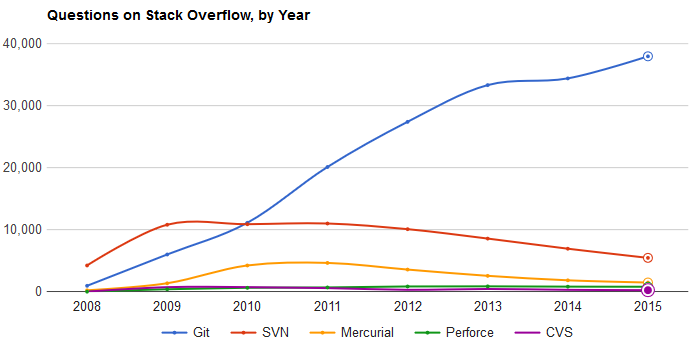
\includegraphics[width=0.78\linewidth]{figures/NumberOfQuestions}
\end{center}
{\tiny source: https://rhodecode.com/}
\end{frame}


\begin{frame}[t]{2. Git (cont'd)}
\framesubtitle{Git workflow}
%\framesubtitle{Git workflow}
%%TODO:plaatje toevoegen 
\vspace*{-9mm}
\begin{tikzpicture}[scale=0.95, every node/.style={scale=0.95}]
% Bubbles
\node[bubble=emclblue] (wd) at (0  , -0.2) {working\\directory};
\node[bubble=emclblue] (sa) at (2.6, -0.2) {staging\\area};
\node[bubble=emclblue] (lc) at (5.2  , -0.2) {local\\ repo};
\node[bubble=emclblue] (rc) at (8.75, -0.2) {remote\\ repo};

\node[above= 0.1 cm of rc,font={\bf}]{Remote};
\node[above= 0.1 cm of sa,font={\bf}]{Local};
% Lines
\foreach \bubble in {wd,sa,lc,rc}
\draw[ultra thick, gray] ($(\bubble.south)-(0,0.25)$)--($(\bubble.south)-(0, 5)$);

% Arrows
\node [arrowstyle=2.6cm, xshift=-0.1cm, yshift=-0.8cm] at ($(wd.south)!0.5!(sa.south)$) {git add};
\node [arrowstyle=2.6cm, xshift=-0.1cm, yshift=-1.3cm] at ($(sa.south)!0.5!(lc.south)$) {git commit};
\node [arrowstyle=3.55cm, xshift=-0.1cm, yshift=-1.8cm] at ($(lc.south)!0.5!(rc.south)$) {git push};
\node [arrowstyle=3.55cm, xshift=0.1cm,  yshift=-2.6cm, shape border rotate=180] at ($(rc.south)!0.5!(lc.south)$) {git fetch};
\node [arrowstyle=5.2cm,xshift=0.1cm, yshift=-3cm, shape border rotate=180] at ($(lc.south)!0.5!(wd.south)$) {git checkout};
\node [arrowstyle=5.2cm,xshift=0.1cm, yshift=-3.8cm, shape border rotate=180] at ($(lc.south)!0.5!(wd.south)$) {git merge};

% Background
\begin{pgfonlayer}{background}
\fill[gray!10]($(lc.north)!0.5!(rc.north)+(0,1)$)rectangle($(lc.south)!0.5!(rc.south)+(4,-5.5)$) ;
\draw[dashed, shorten <=-1.5cm] ($(lc.south)!0.5!(rc.south)+(0,0.5)$)--($(lc.south)!0.5!(rc.south)-(0,5.5)$);
\end{pgfonlayer}
\end{tikzpicture}

\end{frame}


\begin{frame}{2. Git (cont'd)}
\begin{itemize}	
\item Git primarily works via the \alert{command line}
\item When you install git for windows an environment is created that includes some of the basic tools that are also available on linux/unix machine including a version \alert{bash}
\item There are a number of GUIs (\alert{GitKraken} seems ok)
\item Git is also supported from a number of other software packages (like \alert{RStudio}) 
\end{itemize}
\end{frame}


\begin{frame}{2. Git (cont'd)}
\begin{itemize}	
\item Git in RStudio
\begin{itemize}	
\item To use Git in RStudio
\item We need to create a \alert{new project}: \\
Files $\rightarrow$ New project ... $\rightarrow$ Version control
\item Or add to \alert{existing project} \\
Tools $\rightarrow$ Version Control $\rightarrow$ Project Setup
\item Click the dropdown box Version control system and select Git
\item There is now a \alert{git tab} in the upper righthand pannel from which we can do the most common operations  
\end{itemize}
\end{itemize}	
\end{frame}


\begin{frame}{3. Shiny}
\begin{itemize}
	\item Shiny is an R package that makes it easy to build \textbf{interactive web apps} straight from \R 
	\item Shiny combines the computational power of \R with the interactivity of the modern web
	\item Shiny apps are easy to write - No web development skills are required
\end{itemize}


%======================================================
\end{frame}
\begin{frame}{3. Shiny (cont'd)}
\begin{itemize}
\item In \redbf{Rstudio}
\vspace{1ex}
\vspace{1ex}
\begin{itemize}
	\item File $\rightarrow$ New File $\rightarrow$ Shiny Web App...
	\item Insert application name
\end{itemize}
\end{itemize}
\end{frame}

\begin{frame}[fragile]{3. Shiny (cont'd)}
\begin{itemize}
\item \redbf{Example I}
\begin{verbatim}
> library(shiny)
> runExample("01_hello")
\end{verbatim}
\end{itemize}
%======================================================
\end{frame}

\begin{frame}[fragile]{3. Shiny (cont'd)}
\begin{itemize}
\item \redbf{Shiny structure}
\begin{itemize}
\item \bluebf{a user interface object (ui)}
\item \bluebf{a server function}
\item \bluebf{a call to the shinyApp function}
\end{itemize}
\end{itemize}
%======================================================
\end{frame}
\begin{frame}{3. Shiny (cont'd)}
\begin{itemize}
\item \redbf{Shiny structure}
\begin{itemize}
\item \bluebf{a user interface object (ui)}: layout and appearance of your app
\item \bluebf{a server function}: instructions that your computer needs to build your app
\item \bluebf{a call to the shinyApp function}: creates Shiny app objects
\end{itemize}
\end{itemize}
%======================================================
\end{frame}
\begin{frame}[fragile]{3. Shiny (cont'd)}
\begin{itemize}
\item \bluebf{Shiny structure}
\nl
\begin{footnotesize}
\begin{code11}
> library(shiny)

# Define UI ----
> ui <- fluidPage(
)

# Define server logic ----
> server <- function(input, output) {
}

# Run the app ----
> shinyApp(ui = ui, server = server)
\end{code11}
\end{footnotesize}
\end{itemize}
\end{frame}
%======================================================\end{frame}


\end{document}
